\section{GridSolvers}
\label{Sec:Solvers}


%-----------------------------------------------------------------------------
The \code{GridSolvers} unit groups together subunits that are used
to solve particular types of differential equations.  Currently, there
are two types of solvers:  a parallel Fast Fourier Transform package (\secref{Sec:GridSolversPfft})
and various solvers for the Poisson equation (\secref{Sec:GridSolversPoisson}).


%-----------------------------------------------------------------------------
\subsection {Pfft}
\label{Sec:GridSolversPfft}
\code{Pfft} is a parallel frame work for computing a Fast Fourier
Transform (FFT) on uniform grids. It can also be combined with the
Multigrid solver described below in \secref{Sec:GridSolversMultigrid} 
to let the composite solver scale to thousands of processors. 

\code{Pfft} has a layered architecture where the lower layer contains
functions implementing basic tasks and primary data structures.  The
upper layer combines pieces from the lowest layer to interface with Flash-X 
and create the parallel transforms. The computational part
of \code{Pfft} is handled by sequential 1-dimensional FFT's, which can be
from a native, vendor supplied scientific library, or from public
domain packages. The current distribution of Flash-X uses \code{fftpack} from
NCAR for the 1-D FFTs, since that package also contains transforms
that are useful with non-periodic boundary conditions. 

The lowest layer has three distinct components.  
The first component  redistributes data. 
It includes routines for distributed transposes
for two and three dimensional data. The second component provides a
uniform interface for FFT calls to hide the details of individual
libraries.  The third component is the data structures. There are global
data structures to keep track of the type of transform, number of data
dimensions, and physical and transform space information about each
dimension. The dimensional information 
includes the start and end point of data 
(useful when the dimension is spread over more than one processor), 
the MPI communicator, the coordinates of the node in
the processor grid etc. The structures also include pointers to the trigonometric
tables and work space needed by the sequential FFT calls. 

The upper layer of PFFT combines the lower layer routines to create
end-to-end transforms in a variety of ways. The available one
dimensional transforms include real-to-complex, complex-to-complex,
sine and cosine transforms. They can be combined to create two or
three dimensional tranforms for different configuration of the domain.
The two dimensional transforms support parallelization of one
dimension (or a one dimensional grid of  processors). 
The three dimensional transforms support one or two dimensional grid of
processors. All transforms must have at least one dimension within the
processor at all times. The data distribution changes during the
computation. However, a complete cycle of forward and inverse
transform restores the data distribution. 

The computation of a forward three dimensional FFT in parallel involves 
following steps :   
\begin {enumerate}
\item Compute 1-D transforms along {\bf x}.
\item Reorder, or transpose from {\bf x-y-z} to {\bf y-z-x}
\item Compute 1-D  transforms along {\bf y}. If the transform along
{\bf x} was real-to-complex, this one must be a complex-to-complex transform.
\item Transpose from {\bf y-z-x} to {\bf z-x-y}
\item Compute 1-D FFTs along {\bf z}. If the transform along {\bf x}
or {\bf y} was real-to-complex, this must be a complex-to-complex transform.
\end {enumerate} 

The inverse transform can be computed by carrying out the steps
described above in reverse order. The more commonly used domain
decomposition in FFT based codes assumes a one dimensional processor grid:

\begin {equation}\label {Eqn:Pfft_slab}
 N_1 \times N_2 \times N_3/P, 
\end {equation} 
where $N_1 \times N_2 \times N_3$ is the  global data size and $P$ is
the number of processors. Here, the first transpose is local, while
the second one is distributed. The internode communication is limited
to one distributed transpose involving all the processors. However,
there are two distinct disadvantages of this distribution  of work: 
\begin {itemize}
\item  The size of the problem imposes an upper limit on the number of 
processors, in that the largest individual dimension is also the
largest number of active processors. A three dimensional problem
is forced to  have modest individual dimensions to fit in the
processor memory.
\item As the machine size grows, the internode exchanges become long
range, and the possibility of contention grows.
\end {itemize}
We have chosen a domain decomposition where each subdomain is a column
of size \begin {eqnarray} \label {Eqn:Pfft_col}
N_1 \times N_2/P_1 \times N_3/P_2 \\ 
P = P_1 \times P_2. \nonumber
\end {eqnarray} 
With this distribution both the transposes are distributed in
parallel. The data exchange along any one processor grid dimension is
a collection of disjointed distributed transposes. Here, the
contention and communication range is reduced, while the volume of
data exchange is unaltered.  The distributed transposes are
implemented using collective {\bf MPI} operation {\bf alltoall}. In a
slabwise distribution, the upper limit on the number of processors is
determined by the smallest of $<N_1,N_2,N_3>$, where as in our
distribution, the upper limit on the number of processors is the
smallest of $<N_1*N_2,N_2*N_3,N_1*N_3>$. 

\subsubsection{Using \code{Pfft}}
\label{Sec:GridSolversUsingPfft}
\code{Pfft} can only be used with a pencil grid, with the constraint
that the number of processors along the \code{IAXIS} must be 1. This
is because all one dimensional transforms are computed locally within
a processor.  However, Flash-X contains a set of data
movement subroutines that generate a usable pencil grid from any UG
grid or any level of a PM grid.  These routines are briefly explained
in Section \ref{Sec:PFFTDataMove}.

During the course of a simulation, \code{Pfft} can be used in two
different modes. In the first mode, every instance of Pfft use will be
exactly identical to every other instance in terms of domain size and
the type of transforms. In this mode, the user can set the runtime
parameter \rpi{Grid/pfft_setupOnce} to true, which enables the
\code{Flash-X} initialization process to also create and initialize all
the data structures of \code{Pfft}. The finalization of the
\code{Pfft} subunit is also done automatically by the \code{Flash-X}
shutdown process in this mode. However, if a simulation needs to use
\code{Pfft} in different configurations at different instances of its
use, then each set of calls to \api{Grid/Grid_pfft} for computing the
transforms must be preceded by a call to \api{Grid/Grid_pfftInit} and
followed by a call to \api{Grid/Grid_pfftFinalize}. In addition, the
runtime parameter \rpi{Grid/pfft_setupOnce} should be set to false.  A
few other helper routines are available in the subunit to allow the
user to query \code{Pfft} about the dimensioning of the domain, and
also to map the Mesh variables from the \code{unk} array to and from
\code{Pfft} compatible (single dimensional) arrays.  \code{Pfft} also
provides the location of wave numbers in the parallel domain;
information that users can utilize to develop their own customized PDE
solvers using FFT based techniques.

\subsubsection{\code{Pfft} data movement subroutines}
\label{Sec:PFFTDataMove}
Mesh reconfiguration subroutines are available to generate a pencil
grid for the \code{Pfft} unit from another mesh configuration.  Two different implementations are
available at
\code{Grid/\-GridSolvers/\-Pfft/\-MeshReconfiguration/\-PtToPt} and
\code{Grid/\-GridSolvers/\-Pfft/\-MeshReconfiguration/\-Collective},
with the \code{PtToPt} implementation being the default.  Both
implementations are able to generate an appropriate pencil grid in UG
and PM mode.  The pencil processor grid is automatically selected, but
can be overridden by passing optional arguments to
\code{Grid_pfftInit}.  In UG mode they are invoked when the number of
processors in the \code{IAXIS} of the \code{Flash-X} grid is greater than one,
and in PM mode they are always invoked.  In PM mode they generate a
pencil grid from a single level of the AMR grid, which may be manually
specified or automatically selected as the maximum level that is
fully-refined (i.e. has blocks that completely cover the computational
domain at this level).

The pencil grid processor topology is stored in an \code{MPI}
communicator, and the communicator may contain fewer processors than are used in the
simulation.  This is to ensure the pencil grid points are never
distributed too finely over the processors, and naturally handles the 
case where the user may wish to obtain a pencil grid at a very coarse
level in the AMR grid.  If there are more blocks
than processors then we are safe to distribute the pencil grid over
{\bf all} processors, otherwise we must remove a number of processors.
Currently, we eliminate those processors that own {\bf zero} \code{Flash-X}
blocks at this level, as this is a simple calculation that can be
computed locally.

Both mesh reconfiguration implementations generate a map describing 
the data movement before moving any grid data.  The map is 
retained between calls to the \code{Pfft} routines and is 
only regenerated when the grid changes.  This avoids repeating 
the same global communications, but means communication buffers are
left allocated between calls to \code{Pfft}.

In the \code{Collective} 
implementation, the map coordinates are used to specify where 
the \code{Flash-X} data is copied into a send communication buffer.  Two 
\code{MPI_Alltoall} calls then move this data to the appropriate
pencil processor at coordinates (J,K).  Here, the first \code{MPI_Alltoall} moves data 
to processor (J,0), and the second \code{MPI_Alltoall} moves data 
to processor (J,K).  The decision to use \code{MPI_Alltoalls}
simplifies the \code{MPI} communication, but leads to very large 
send / receive communication buffers on each processor which consume:

\begin{verbatim}
Memory(bytes) = sizeof(REAL) * total grid points at solve level * 2
\end{verbatim}

The \code{PtToPt} implementation consumes less memory compared to the
\code{Collective} implementation, and communicates using point to
point \code{MPI} messages.  It is based upon using nodes in a linked
list which contain metadata (a map) and a communication buffer for a
single block fragment.  There are two linked lists: one for the
\code{Flash-X} block fragments and one for \code{Pfft} block fragments.
Metadata information about each \code{Flash-X} block fragment is placed
in separate messages and sent using \code{MPI_Isend} to the
appropriate destination pencil grid processor.

Each destination pencil grid processor repeatedly invokes
\code{MPI_Iprobe} using \code{MPI_ANY_SOURCE}, and creates a node in
its \code{Pfft} list whenever it discovers a message.  The \code{MPI}
message is received into a metadata region of the freshly allocated
node, and a communication buffer is also allocated according to the
size specified in the metadata.  The pencil processor continues
probing for messages until the cumulative size of its node's
communication buffers is equal to the pencil grid points it has been
assigned.  At this stage, grid data is communicated by traversing the
\code{Pfft} list and posting \code{MPI_Irecvs}, and then traversing
the \code{Flash-X} list and sending block fragment using
\code{MPI_Isends}.  After performing \code{MPI_Waits}, the received data in the 
nodes of the \code{Pfft} list is copied into internal \code{Pfft} arrays.

Note, the linked list is constructed using an include file stored at
\code{flashUtilities/\-datastructures/\-linkedlist}.  The file is named
\code{ut_listMethods.includeF90} and is meant to be included in any
\code{Fortran90} module to create lists with nodes of
a user-defined type.  Please see the README file, and the unit test
example at \code{flashUtilities/\-datastructures/\-linkedlist/\-UnitTest}.


\subsubsection{Unit Test}
\label{Sec:GridSolversPfftUnitTests}

The unit test for Pfft solver solves the following equation:
\begin{equation}
\label{Eqn:pfft Poisson}
\nabla^2({\bf F})=-13.0*\cos2x*\sin3y
\end{equation}
The simplest analytical solution of this equation assuming no
constants is
\begin{equation}
F=\cos2x*\sin3y
\end{equation}
We discretize the domain by assuming $xmin,ymin,zmin=0$, and
$xmax,ymax,zmax=2\pi$. The equation satisfies periodic boundary
conditions in this formulation and FFT based poisson solve techniques
can be applied. In the unit test we initialize one variable of the
solution data with the function $F$, and another one
with the right hand side of  \eqref{Eqn:pfft Poisson}. We
compute the forward real-to-complex transform of the solution data
variable that is initialized with the right hand side of \eqref{Eqn:pfft
Poisson}.  This variable is then divided by  
$({k_i}^2+{k_j}^2+{k_k}^2)$ where ${k_i, k_j}$ and ${k_k}$ are the
wavenumbers at any point {i,j,k} in the domain. An inverse complex-to-real
transform after the division should give the function $F$ as
result. Hence the unit test is considered successful if both the
variables have matching values within the specified tolerance.

\subsection{Poisson equation}
\label{Sec:GridSolversPoisson}

The \code{GridSolvers} subunit contains several different algorithms
for solving the general Poisson equation for a potential $\phi({\bf
x})$ given a source $\rho({\bf x})$ 
\begin{equation}
\label{Eqn:general Poisson}
\nabla^2\phi({\bf x}) = \alpha\rho({\bf x})\ .
\end{equation}
Here $\alpha$ is a constant that depends upon the application.  For example,
when the gravitational Poisson equation is being solved, $\rho({\bf x})$ is
the mass density, $\phi({\bf x})$ is the gravitational potential, and
$\alpha = 4\pi G$, where $G$ is Newton's gravitational constant.







\subsubsection{Multipole Poisson solver (original version)}
\label{Sec:GridSolversMultipole}
This section describes the multipole Poisson solver that has been
included in all the past releases of Flash-X. It is included in the
current release also, however, certain limitations found in this
solver lead to a new implementation described in
\secref{Sec:GridSolversMultipoleImproved}. This version is retained in
\flashx, because the new version is missing 
the ability to treat a non-zero minimal radius for spherical
geometries and the ability to specify a point mass contribution to the
potential. This will be implemented for the next coming release. 

The multipole Poisson solver is appropriate for spherical or nearly-spherical
source distributions with isolated boundary conditions (M{\"u}ller (1995)).
It currently works in 1D and 2D spherical, 2D axisymmetric cylindrical ($r,z$), and
3D Cartesian and axisymmetric geometries. Because of the imposed symmetries,
in the 1D spherical case, only the monopole term ($\ell = 0$) makes sense,
while in the axisymmetric and 2D spherical cases, only the $m = 0$ moments are used (\ie, the
basis functions are Legendre polynomials).

The multipole algorithm consists of the following steps.
First, find the center of mass ${\bf x}_{\rm cm}$
\begin{equation}
{\bf x}_{\rm cm} = {\int d^3{\bf x}\,{\bf x}\rho({\bf x}) \over
                    \int d^3{\bf x}\,\rho({\bf x})}\ .
\end{equation}
We will take ${\bf x}_{\rm cm}$ as our origin.  In integral form, Poisson's
(\eqref{Eqn:general Poisson}) is
\begin{equation}
\label{Eqn:Poisson integral}
\phi({\bf x}) = -{\alpha\over 4\pi}\int d^3{\bf x}'\,{\rho({\bf x}')\over
                |{\bf x} - {\bf x}'|}\ .
\end{equation}
The Green's function for this equation satisfies the relationship
\begin{equation}
\label{Eqn:Green}
{1\over |{\bf x} - {\bf x}'|} =
  4\pi\sum_{\ell=0}^\infty \sum_{m=-\ell}^\ell {1\over 2\ell+1}
  {r_<^\ell\over r_>^{\ell+1}}
  Y_{\ell m}^*(\theta',\varphi') Y_{\ell m}(\theta,\varphi)\ ,
\end{equation}
where the components of ${\bf x}$ and ${\bf x}'$ are expressed in
spherical coordinates $(r,\theta,\varphi)$ about ${\bf x}_{\rm cm}$, and
\begin{eqnarray}
r_< &\equiv& \min\{ |{\bf x}|, |{\bf x}'| \} \\
\nonumber
r_> &\equiv& \max\{ |{\bf x}|, |{\bf x}'| \}\ .
\end{eqnarray}
Here $Y_{\ell m}(\theta,\varphi)$ are the spherical harmonic functions
\begin{equation}
Y_{\ell m}(\theta,\varphi) \equiv
  (-1)^m \sqrt{ {2\ell+1\over 4\pi} {(\ell-m)!\over (\ell+m)!} }
  P_{\ell m}(\cos\theta) e^{im\varphi}\ .
\end{equation}
$P_{\ell m}(x)$ are Legendre polynomials.
Substituting \eqref{Eqn:Green} into
\eqref{Eqn:Poisson integral}, we obtain
\begin{eqnarray}
\label{Eqn:Multipole_poisint2}
\phi({\bf x}) &=& -\alpha
  \sum_{\ell=0}^\infty \sum_{m=-\ell}^\ell {1\over 2\ell+1}
  \Biggl\{
  Y_{\ell m}(\theta,\varphi) \times \\
\nonumber
  &&
  \left[ r^\ell \int_{r<r'} d^3{\bf x}' {\rho({\bf x}')
                   Y_{\ell m}^*(\theta',\varphi')\over {r'}^{\ell+1}} +
         {1\over r^{\ell+1}} \int_{r>r'} d^3{\bf x}' \rho({\bf x}')
                   Y_{\ell m}^*(\theta',\varphi') {r'}^\ell \right]\Biggr\} \ .
\end{eqnarray}
In practice, we carry out the first summation
up to some limiting multipole $\ell_{\rm max}$.
By taking spherical harmonic expansions about the center of mass, we
ensure that the expansions are dominated by low-multipole terms, so
that for a given value of $\ell_{\rm max}$, the error created by
neglecting high-multipole terms is minimized.
Note that the product of spherical harmonics in \eqref{Eqn:Multipole_poisint2} is
real-valued
\begin{eqnarray}
\sum_{m=-\ell}^\ell Y_{\ell m}^*(\theta',\varphi') Y_{\ell m}(\theta,\varphi)&=&
  {2\ell+1\over 4\pi} \Biggl[ P_{\ell 0}(\cos\theta) P_{\ell 0}(\cos\theta') +
  \\
\nonumber
  &&
  2\sum_{m=1}^\ell {(\ell-m)!\over (\ell+m)!}
  P_{\ell m}(\cos\theta)P_{\ell m}(\cos\theta')
  \cos\left(m(\varphi-\varphi')\right)
  \Biggr]\ .
\end{eqnarray}
Using a trigonometric identity to split up the last cosine in this expression
and substituting for the inner sums in \eqref{Eqn:Multipole_poisint2},
we obtain
\begin{eqnarray}
\label{Eqn:multipole potential}
\nonumber
\phi({\bf x}) &=& -{\alpha\over 4\pi}
                   \sum_{\ell=0}^\infty P_{\ell 0}(\cos\theta)\left[
  r^\ell \mu^{\rm eo}_{\ell 0}(r) +
  {1\over r^{\ell+1}} \mu^{\rm ei}_{\ell 0}(r) \right] - \\
  &&
  {\alpha\over 2\pi}
  \sum_{\ell=1}^\infty \sum_{m=1}^\ell P_{\ell m}(\cos\theta)\biggl[
  (r^\ell \cos m\varphi) \mu^{\rm eo}_{\ell m}(r) +
  (r^\ell \sin m\varphi) \mu^{\rm oo}_{\ell m}(r) + \\
\nonumber
  &&\qquad\qquad\qquad\qquad\qquad
  {\cos m\varphi\over r^{\ell+1}} \mu^{\rm ei}_{\ell m}(r) +
  {\sin m\varphi\over r^{\ell+1}} \mu^{\rm oi}_{\ell m}(r) \biggr]\ .
\end{eqnarray}
The even (e)/odd (o), inner (i)/outer (o) source moments in this expression are
defined to be
\begin{eqnarray}
\label{Eqn:moments1}
\mu^{\rm ei}_{\ell m}(r) &\equiv&
  {(\ell-m)!\over (\ell+m)!} \int_{r>r'} d^3{\bf x}'\,
  {r'}^\ell \rho({\bf x}') P_{\ell m}(\cos\theta') \cos m\varphi' \\
\mu^{\rm oi}_{\ell m}(r) &\equiv&
  {(\ell-m)!\over (\ell+m)!} \int_{r>r'} d^3{\bf x}'\,
  {r'}^\ell \rho({\bf x}') P_{\ell m}(\cos\theta') \sin m\varphi' \\
\mu^{\rm eo}_{\ell m}(r) &\equiv&
  {(\ell-m)!\over (\ell+m)!} \int_{r<r'} d^3{\bf x}'\,
  {\rho({\bf x}')\over {r'}^{\ell+1}} P_{\ell m}(\cos\theta') \cos m\varphi'
  \\
\label{Eqn:moments4}
\mu^{\rm oo}_{\ell m}(r) &\equiv&
  {(\ell-m)!\over (\ell+m)!} \int_{r<r'} d^3{\bf x}'\,
  {\rho({\bf x}')\over {r'}^{\ell+1}} P_{\ell m}(\cos\theta') \sin m\varphi'
  \ .
\end{eqnarray}
The procedure is thus to compute the moment integrals 
(\eqref{Eqn:moments1} $-$ \eqref{Eqn:moments4})
for a given source field $\rho({\bf x})$, and then to use these moments
in \eqref{Eqn:multipole potential} to compute the
potential.

In practice, the above procedure must take account of the fact that the
source and the potential are assumed to be cell-averaged
quantities discretized on a block-structured mesh with varying cell size.
Also, because of the radial dependence of the multipole moments of the
source function, these moments must be tabulated as functions of distance from
${\bf x}_{\rm cm}$, with an implied discretization.  The solver allocates
storage for moment samples spaced a distance $\Delta$ apart in radius
\begin{eqnarray}
\mu^{\rm ei}_{\ell m,q}\equiv \mu^{\rm ei}_{\ell m}(q\Delta) &&
\mu^{\rm eo}_{\ell m,q}\equiv \mu^{\rm eo}_{\ell m}((q-1)\Delta) \\
\mu^{\rm oi}_{\ell m,q}\equiv \mu^{\rm oi}_{\ell m}(q\Delta) &&
\mu^{\rm oo}_{\ell m,q}\equiv \mu^{\rm oo}_{\ell m}((q-1)\Delta)\ .
\end{eqnarray}
The sample index $q$ varies from 0 to $N_q$ ($\mu^{\rm eo}_{\ell m,0}$ and
$\mu^{\rm oo}_{\ell m,0}$ are not used).  The sample spacing $\Delta$ is
chosen to be one-half the geometric mean of the $x$, $y$, and $z$ cell spacings
at the highest level of refinement, and $N_q$ is chosen to be large enough
to span the diagonal of the computational volume with samples.

Determining the contribution of individual
cells to the tabulated moments requires some care.  To reduce the error
caused by the grid geometry, in each cell $ijk$
an optional subgrid can be establish (see \rpi{Grid/mpole_subSample})
consisting of $N'$ points at the locations
${\bf x}'_{i'j'k'}$, where
\begin{eqnarray}
x'_{i'} = x_i + (i'-0.5(N'-1)){\Delta x_i\over {N'}}\ ,&&
  i' = 0\ldots {N'}-1 \\
y'_{j'} = y_j + (j'-0.5(N'-1)){\Delta y_j\over {N'}}\ ,&&
  j' = 0\ldots {N'}-1 \\
z'_{k'} = z_k + (k'-0.5(N'-1)){\Delta z_k\over {N'}}\ ,&&
  k' = 0\ldots {N'}-1 \ ,
\end{eqnarray}
and where ${\bf x}_{ijk}$ is the center of cell $ijk$.  (For clarity, we have
omitted $ijk$ indices on ${\bf x}'$ as well as all block indices.)
For each subcell, we assume $\rho({\bf x}'_{i'j'k'})\approx\rho_{ijk}$
and then apply
\begin{eqnarray}
\label{Eqn:discmoments1}
\mu^{\rm ei}_{\ell m,q\ge q'} &\leftarrow& \mu^{\rm ei}_{\ell m,q\ge q'} +
  {(\ell-m)!\over (\ell+m)!} {\Delta x_i\Delta y_j\Delta z_k\over {N'}^3}
  {r'}_{i'j'k'}^\ell \rho({\bf x}'_{i'j'k'}) P_{\ell m}(\cos\theta'_{i'j'k'})
  \cos m\varphi'_{i'j'k'} \\
\mu^{\rm oi}_{\ell m,q\ge q'} &\leftarrow& \mu^{\rm oi}_{\ell m,q\ge q'} +
  {(\ell-m)!\over (\ell+m)!} {\Delta x_i\Delta y_j\Delta z_k\over {N'}^3}
  {r'}_{i'j'k'}^\ell \rho({\bf x}'_{i'j'k'}) P_{\ell m}(\cos\theta'_{i'j'k'})
  \sin m\varphi'_{i'j'k'} \\
\mu^{\rm eo}_{\ell m,q\le q'} &\leftarrow& \mu^{\rm eo}_{\ell m,q\le q'} +
  {(\ell-m)!\over (\ell+m)!} {\Delta x_i\Delta y_j\Delta z_k\over {N'}^3}
  {\rho({\bf x}'_{i'j'k'})\over {r'}_{i'j'k'}^{\ell+1}}
  P_{\ell m}(\cos\theta'_{i'j'k'})
  \cos m\varphi'_{i'j'k'} \\
\label{Eqn:discmoments4}
\mu^{\rm oo}_{\ell m,q\le q'} &\leftarrow& \mu^{\rm oo}_{\ell m,q\le q'} +
  {(\ell-m)!\over (\ell+m)!} {\Delta x_i\Delta y_j\Delta z_k\over {N'}^3}
  {\rho({\bf x}'_{i'j'k'})\over {r'}_{i'j'k'}^{\ell+1}}
  P_{\ell m}(\cos\theta'_{i'j'k'}) \sin m\varphi'_{i'j'k'}
  \ ,
\end{eqnarray}
where
\begin{equation}
q' = \left\lfloor{|{\bf x}'_{i'j'k'} }| \over {\Delta}
     \right\rfloor + 1
\end{equation}
is the index of the radial sample within which the subcell center lies.
These expressions introduce (hopefully) small errors when compared to
(\eqref{Eqn:moments1}) $-$ (\ref{Eqn:moments4}), because the
subgrid volume elements are not spherical. These
errors are greatest when $r' \sim \Delta x$; hence, using a subgrid
reduces the amount of source affected by these errors.
An error of order $\Delta^2$ is also introduced by assuming the source
profile within each cell to be flat.
Note that the total source computed by this method ($\mu^{\rm ei}_{\ell m,N_q}$)
is exactly equal to the total implied by $\rho_{ijk}$.

Another way to reduce grid geometry errors when using the multipole
solver is to modify the AMR refinement criterion to refine all blocks
containing the center of mass (in addition to other criteria that may
be used, such as the second-derivative criterion supplied with \Paramesh).
This ensures that the center-of-mass point is maximally refined at all
times, further restricting the volume which contributes errors to the
moments because $r' \sim \Delta x$.

The default value of $N'$ is 1; note that large values of this
parameter very quickly increase the amount of time required to evaluate
the multipole moments (as ${N'}^3$). In order to speed up the moment
summations, the sines and cosines in
(\eqref{Eqn:discmoments1}) $-$ (\ref{Eqn:discmoments4}) are evaluated using
trigonometric recurrence relations, and the factorials are pre-computed
and stored at the beginning of the run.

When computing the cell-averaged potential, we again employ a subgrid, but
here the subgrid points fall on cell boundaries to improve the continuity
of the result.  Using $N'+1$ subgrid points per dimension, we have
\begin{eqnarray}
x'_{i'} = x_i + (i'-0.5N')){\Delta x_i\over {N'}}\ ,&&
  i' = 0\ldots {N'} \\
y'_{j'} = y_j + (j'-0.5N')){\Delta y_j\over {N'}}\ ,&&
  j' = 0\ldots {N'} \\
z'_{k'} = z_k + (k'-0.5N')){\Delta z_k\over {N'}}\ ,&&
  k' = 0\ldots {N'} \ .
\end{eqnarray}
The cell-averaged potential in cell $ijk$ is then
\begin{equation}
\phi_{ijk} = {1\over {N'}^3} \sum_{i'j'k'} \phi({\bf x}'_{i'j'k'})\ ,
\end{equation}
where the terms in the sum are evaluated via 
\eqref{Eqn:multipole potential} up to the limiting multipole order
$\ell_{\rm max}$.

\begin{comment}
\begin{flashtip}
In \flashx, two different parameters were available to control subsampling.
In \flashx, the sub-sampling is made consistent with the use of only one
runtime parameter \rpi{Grid/mpole_subSample} to avoid excessive wasted computation
in one section of the calculation.
The default value of \code{mpole_subSample} is 1; meaning no subsampling is performed
by default and the code runs much faster.  Should additional accuracy be required, increase
this runtime parameter.
\end{flashtip}
\end{comment}


\subsubsection{Multipole Poisson solver (improved version)}
\label{Sec:GridSolversMultipoleImproved}

The multipole Poisson solver is based on a multipolar expansion of the source (mass for gravity,
for example) distribution around a conveniently chosen center of expansion. The angular number
$L$ entering this expansion is a measure of how detailed the description of the source
distribution will be on an angular basis. Higher $L$ values mean higher angular resolution with
respect to the center of expansion. The multipole Poisson solver is thus appropriate for spherical
or nearly-spherical source distributions with isolated boundary conditions. For problems which
require high spatial resolution throughout the entire domain (like, for example, galaxy collision
simulations), the multipole Poisson solver is less suited, unless one is willing to go to extremely
(computationally unfeasible) high $L$ values. For stellar evolution, however, the multipole
Poisson solver is the method of choice.
\par
The new implementation of the multipole Poisson solver is located in the directory
\begin{codeseg}
source/Grid/GridSolvers/Multipole_new.
\end{codeseg}
This implementation improves upon the original implemention in many ways:
i) efficient memory layout 
ii) elimination of numerical over- and underflow
errors for large angular momenta when using astrophysical
(dimensions $\approx 10^9$) domains
iii) elimination of subroutine call overhead (1 call per cell),
iv) minimization of error due to non-statistical distributions of
moments near the multipolar origin. The following paragraphs explain
the new approach to the multipole solver and an explanation of the
above improvements. Details about the theory of the new implementation of the Poisson solver
can be found in Couch et al.~(2013).
\par
The multipole Poisson solver is appropriate for spherical or nearly-spherical
source distributions with isolated boundary conditions. It currently works in
1D spherical, 2D spherical, 2D cylindrical, 3D Cartesian and 3D cylindrical. Symmetries
can be specified for the 2D spherical and 2D cylindrical cases (a horizontal symmetry plane
along the radial axis) and the 3D Cartesian case (assumed axisymmetric property).
Because of the radial symmetry in the 1D spherical case, only the monopole term
($\ell = 0$) contributes, while for the 3D Cartesian axisymmetric, the 2D cylindrical
and 2D spherical cases only the $m = 0$ moments need to be used (the other $m\neq 0$
moments effectively cancel out).
\par
The multipole algorithm consists of the following steps. First, the center of
the multipolar expansion ${\bf x}_{\rm cen}$ is determined via density-squared weighted
integration over position:
\begin{equation}
{\bf x}_{\rm cen} = {\int {\bf x}\rho^2({\bf x})\,d{\bf x} \over
                    \int \rho^2({\bf x})\,d{\bf x}}.
\end{equation}
We will take ${\bf x}_{\rm cen}$ as our origin.  In integral form, Poisson's
equation (\ref{Eqn:general Poisson}) becomes
\begin{equation}
\label{Eqn:PoissonIntegral}
\phi({\bf x}) = -{\alpha\over 4\pi}\int {\rho({\bf x}')\over
                |{\bf x} - {\bf x}'|}\,d{\bf x}'.
\end{equation}
The inverse radial distance part can be expanded in terms of Legendre
polynomials
\begin{equation}
\label{Eqn:Inverse distance Legendre}
{1\over |{\bf x} - {\bf x}'|} = \sum_{\ell=0}^\infty
{x_<^\ell\over x_>^{\ell+1}}P_\ell (\cos\gamma),
\end{equation}
where $x_<$ ($x_>$) indicate the smaller (larger) of the magnitudes
and $\gamma$ denotes the angle between ${\bf x}$ and ${\bf x}'$. Note, that this
definition includes those cases where both magnitudes are equal. The expansion
is always convergent if $\cos\gamma <1$. Expansion of the Legendre polynomials
in terms of spherical harmonics gives
\begin{equation}
\label{Eqn:Legendre spherical harmonics}
P_\ell (\cos\gamma) = {4\pi\over 2\ell+1}\sum_{m=-\ell}^{+\ell}
Y_{\ell m}^*(\theta',\phi') Y_{\ell m}(\theta,\phi),
\end{equation}
where $\theta,\phi$ and $\theta',\phi'$ are the spherical angular components of
${\bf x}$ and ${\bf x}'$ about ${\bf x}_{\rm cen}$.
Defining now the regular $R_{\ell m}$ and irregular $I_{\ell m}$ solid
harmonic functions
\begin{eqnarray}
R_{\ell m}(x_<) & = & \sqrt{{4\pi\over {2\ell+1}}}x_<^\ell Y_{\ell m}(\theta,\phi) \\
I_{\ell m}(x_>) & = & \sqrt{{4\pi\over {2\ell+1}}}{Y_{\ell m}(\theta,\phi)\over x_>^{\ell+1}},
\end{eqnarray}
we can rewrite Eq.(\ref{Eqn:PoissonIntegral}) in the form
\begin{equation}
\label{Eqn:Poisson solid harmonics}
\phi({\bf x}) = -{\alpha\over 4\pi}
\int \sum_{\ell m}R_{\ell m}(x_<)I_{\ell m}^*(x_>)\rho({\bf x}')\,d{\bf x}',
\end{equation}
where the summation sign is a shorthand notation for the double sum over all the
allowed $\ell$ and $m$ values. In Flash-X both the source and the potential are
assumed to be cell-averaged quantities discretized on a block-structured mesh with
varying cell size. The integration must hence be replaced by a summation over all 
leaf cells
\begin{equation}
\label{Eqn:Poisson discrete incorrect}
\phi(q) = -{\alpha\over 4\pi}
\sum_{q'} \sum_{\ell m}R_{\ell m}(q_<)I_{\ell m}^*(q_>)m(q'),
\end{equation}
where $m$ denotes the cell's mass. Note, that the symbol $q$ stands for cell index as well
as its defining distance position from the expansion center in the computational domain.
This discrete Poisson equation is incorrect. It contains the divergent $q'=q$ term on
the rhs. The $q'=q$ contribution to the potential corresponds to the cell self potential
$\phi_{Self}(q)$ and is divergent in our case because all the cell's mass is assumed to be
concentrated at the cell's center. The value of this divergent term can easily be calculated
from Eq.(\ref{Eqn:Inverse distance Legendre}) by setting $\cos\gamma = 1$:
\begin{eqnarray}
\phi_{Self}(q) & = &  m(q){L+1\over x_q},
\end{eqnarray}
where $m$ is the cell's mass, $L$ the highest angular number considered in the expansion
and $x_q$ the radial distance of the cell center from the expansion center. To avoid this divergence
problem, we evaluate the potentials on each face of the cell and form the average of all
cell face potentials to get the cell center potential. Eq.(\ref{Eqn:Poisson discrete incorrect})
will thus be replaced by
\begin{equation}
\phi(q) = {1\over n_F} \sum_{F} \phi({\bf x}_F)
\end{equation}
and
\begin{equation}
\label{Eqn:Poisson discrete correct}
\phi({\bf x}_F) = -{\alpha\over 4\pi}
\sum_{q'} \sum_{\ell m}R_{\ell m}([q',x_F]_<)I_{\ell m}^*([q',x_F]_>)m(q'),
\end{equation}
where ${\bf x}_F$ is the cell face radial distance from the expansion center and $[q',x_F]_<$ denotes the
larger of the magnitudes between the cell center radial distance $q'$ and the cell face radial distance $x_F$.
Splitting the summation over cells in two parts
\begin{equation}
\label{Eqn:Poisson discrete correct 1}
\phi({\bf x}_F) = -{\alpha\over 4\pi}\left\{
\sum_{q'\leq x_F} \sum_{\ell m}\left[R_{\ell m}(q')m(q')\right]I_{\ell m}^*({\bf x}_F)
+ \sum_{q'>x_F} \sum_{\ell m}R_{\ell m}({\bf x}_F)\left[I_{\ell m}^*(q')m(q')\right]\right\},
\end{equation}
and defining the two moments
\begin{eqnarray}
M^R_{\ell m}({\bf x}_F) & = & \sum_{q'\leq x_F} R_{\ell m}(q')m(q') \label{Eqn:Moment definition 1} \\
M^I_{\ell m}({\bf x}_F) & = & \sum_{q'>x_F} I_{\ell m}(q')m(q'),\label{Eqn:Moment definition 2}
\end{eqnarray}
we obtain
\begin{equation}
\label{Eqn:Poisson discrete correct 2}
\phi({\bf x}_F) = -{\alpha\over 4\pi}\left[
\sum_{\ell m}M^R_{\ell m}({\bf x}_F)I_{\ell m}^*({\bf x}_F)
+ \sum_{\ell m}M^{I*}_{\ell m}({\bf x}_F)R_{\ell m}({\bf x}_F)\right]
\end{equation}
and using vector notation
\begin{equation}
\label{Eqn:Poisson discrete correct 3}
\phi({\bf x}_F) = -{\alpha\over 4\pi}\left[
{\bf M}^R({\bf x}_F)\cdot {\bf I}^*({\bf x}_F) + {\bf M}^{I*}({\bf x}_F)\cdot {\bf R}({\bf x}_F)
\right].
\end{equation}
\par
We now change from complex to real formulation. We state this for the regular
solid harmonic functions, the same reasoning being applied to the irregular
solid harmonic functions and all their derived moments. The regular solid
harmonic functions can be split into a real and imaginary part
\begin{equation}
\label{Eqn:Solid harmonics real}
R_{\ell m} = R_{\ell m}^c + i\,R_{\ell m}^s.
\end{equation} 
The labels 'c' and 's' are shorthand notations for 'cosine' and 'sine',
reflecting the nature of the azimuthal function of the corresponding real
spherical harmonics. When inserting (\ref{Eqn:Solid harmonics real}) into
(\ref{Eqn:Poisson discrete correct 3}) all cosine and sine mixed terms of the
scalar products cancel out. Also, due to the symmetry relations
\begin{eqnarray}
R_{\ell,-m}^c & = & (-1)^m R_{\ell m}^c \\
R_{\ell,-m}^s & = & -(-1)^m R_{\ell m}^s
\end{eqnarray} 
we can restrict ourselves to the following polar angle number ranges
\begin{eqnarray}
c & : & \ell\geq 0\;\;,\;\;\ell\geq m \geq 0 \\
s & : & \ell\geq 1\;\;,\;\;\ell\geq m \geq 1.
\end{eqnarray}
The real formulation of (\ref{Eqn:Poisson discrete correct 3}) becomes then
\begin{equation}
\label{Eqn:Poisson discrete correct real}
\phi({\bf x}_F) = -{\alpha\over 4\pi}\left\{
\left[\begin{array}{l}
{\bf M}^{Rc}({\bf x}_F) \\
{\bf M}^{Rs}({\bf x}_F)
\end{array}\right]
\cdot {\bf \Delta}
\left[\begin{array}{l}
{\bf I}^c({\bf x}_F) \\
{\bf I}^s({\bf x}_F)
\end{array}\right]
+
\left[\begin{array}{l}
{\bf M}^{Ic}({\bf x}_F) \\
{\bf M}^{Is}({\bf x}_F)
\end{array}\right]
\cdot {\bf \Delta}
\left[\begin{array}{l}
{\bf R}^c({\bf x}_F) \\
{\bf R}^s({\bf x}_F)
\end{array}\right]\right\},
\end{equation}
which, when compared to (\ref{Eqn:Poisson discrete correct 3}), shows, that all vectors now
contain a cosine and a sine section. The ${\bf \Delta}$ matrix is a diagonal matrix whose elements
are equal to 2 for $m\neq 0$ and 1 otherwise, i.e.:
\begin{equation}
\label{Eqn:Delta matrix}
{\bf \Delta} = diag(2-\delta_{m0}).
\end{equation}
The recursion relations for calculating the solid harmonic vectors are
\begin{eqnarray}
R_{00}^c & = & 1 \label{Eqn:Regular Recurrence} \\
R_{\ell\ell}^c & = & - {xR_{\ell-1,\ell-1}^c-yR_{\ell-1,\ell-1}^s\over 2\ell}\\
R_{\ell\ell}^s & = & - {yR_{\ell-1,\ell-1}^c+xR_{\ell-1,\ell-1}^s\over 2\ell}\\
R_{\ell m}^{c/s} & = & {(2\ell - 1)zR_{\ell-1,m}^{c/s}-r^2R_{\ell-2,m}^{c/s}
                       \over (\ell + m)(\ell - m)},\;\;\;0\leq m <\ell
\end{eqnarray}
and
\begin{eqnarray}
I_{00}^c & = & {1\over r} \\
I_{\ell\ell}^c & = & - (2\ell-1){xI_{\ell-1,\ell-1}^c-yI_{\ell-1,\ell-1}^s\over r^2} \\
I_{\ell\ell}^s & = & - (2\ell-1){yI_{\ell-1,\ell-1}^c+xI_{\ell-1,\ell-1}^s\over r^2} \\
I_{\ell m}^{c/s} & = & {(2\ell - 1)zI_{\ell-1,m}^{c/s}-\left[(\ell-1)^2-m^2\right]
                       I_{\ell-2,m}^{c/s}\over r^2},\;\;\;0\leq m <\ell
\label{Eqn:Irregular Recurrence}
\end{eqnarray}
in which $x,y,z$ are the cartesian location coordinates of the cell face and $r^2=x^2+y^2+z^2$.
For geometries depending on polar angles one must first calculate the corresponding cartesian
coordinates for each cell before applying the recursions. In Flash-X, the order of the two cosine
and sine components for each solid harmonic vector is such that $\ell$ precedes $m$.
This allows buildup of the vectors with maximum number of unit strides. The same
applies of course for the assembly of the moments. For 2D cylindrical and 2D spherical geometries
only the $m=0$ parts of both recursions are needed, involving only the cartesian $z$ coordinate
and $r^2$. Symmetry along the radial axes of these 2D geometries inflicts only the sign change
$z\rightarrow -z$, resulting in the symmetry relations $R_{\ell 0}^c\rightarrow R_{\ell 0}^c$ for
even $\ell$ and $R_{\ell 0}^c\rightarrow -R_{\ell 0}^c$ for odd $\ell$, the same holding for the
irregular solid harmonic vector components. Thus symmetry in 2D can effectively be treated
by halving the domain size and multiplying each even $\ell$ moments by a factor of 2 while setting
the odd $\ell$ moments equal to 0. For 3D cartesian geometries introduction of symmetry
is far more complicated since all $m$ components need to be taken into account. It is not
sufficient to simply reduce the domain to the appropriate size and multiply the moments
by some factor, but rather one would have to specify the exact symmetry operations intended
(generators of the symmetry group $O_h$ or one of its subgroups) in terms of their effects
on the $x,y,z$ cartesian basis. The resulting complications in calculating symmetry adapted moments
outweighs the computational gain that can be obtained from it. Options for 3D symmetry are
thus no longer available in the improved Flash-X multipole solver. The 'octant' symmetry option
from the old multipole solver, using only the monopole $\ell=0$ term, was too restrictive in
its applicability (exact only for up to angular momenta $\ell =3$ due to cancellation of the
solid harmonic vector components).
\par
From the above recursion relations (\ref{Eqn:Regular Recurrence}-\ref{Eqn:Irregular Recurrence}),
the solid harmonic vector components are functions
of $x^iy^jz^k$ monomials, where $i+j+k=\ell$ for the ${\bf R}$ and (formally)
$i+j+k=-(\ell+1)$ for the ${\bf I}$. For large astrophysical coordinates and large $\ell$ values this leads
to potential computational over- and underflow. To get independent of the size of both
the coordinates and $\ell$ we introduce a damping factor $Dx,Dy,Dz$ for the coordinates
for each solid harmonic type before entering the recursions. $D$ will be chosen such that for the
highest specified $\ell=L$ we will have approximately a value close to 1 for both
solid harmonic components:
\begin{eqnarray}
R^{c/s}_{Lm} & \approx & 1 \label{Eqn:Damping condition 1} \\
I^{c/s}_{Lm} & \approx & 1.\label{Eqn:Damping condition 2}
\end{eqnarray}
This ensures proper handling of size at the solid harmonic function evaluation level and one
does not have to rely on size cancellations at a later stage when evaluating the potential via
Eq.(\ref{Eqn:Poisson discrete correct real}). We next state the evaluation of the
damping factor $D$. Due to the complicated nature of the recursions, the first step is to
find solid harmonic components which have a simple structure. To do this, consider a cell
face with $x,y=0$ and $z\neq 0$. Then $r^2=z^2$, $|z|=r$ and only the $m=0$ components are
different from zero. An explicit form can be stated for the absolute values of these
components in terms of $r$:
\begin{eqnarray}
\label{Eqn:Regular solid harmonic xy0}
|R_{\ell 0}| & = & {r^\ell\over \ell!} \\
|I_{\ell 0}| & = & {\ell!\over r^{\ell+1}}. \label{Eqn:Irregular solid harmonic xy0}
\end{eqnarray}
Since $r=\sqrt{x^2+y^2+z^2}$, damping of the coordinates with $D$ results in a damped
radial cell face distance $Dr$. Inserting this result into (\ref{Eqn:Regular solid harmonic xy0})
and (\ref{Eqn:Irregular solid harmonic xy0})
and imposing conditions (\ref{Eqn:Damping condition 1}) and (\ref{Eqn:Damping condition 2})
results in
\begin{eqnarray}
\label{Eqn:Damping components}
D_R = {1\over r}\sqrt[L]{L!} & \approx & {1\over r}{L\over e}\sqrt[2L]{2\pi L}\\
D_I = {1\over r}\sqrt[L+1]{L!} & \approx & {1\over r}{L\over e}\sqrt[2L+2]{{2\pi e^2\over L}},
\end{eqnarray}
where the approximate forms are obtained by using Stirling's factorial approximation
formula for large $L$. In Flash-X only the approximate forms are computed for $D_R$ and $D_I$
to avoid having to deal with factorials of large numbers.
\par
From the moment defining equations (\ref{Eqn:Moment definition 1}) and (\ref{Eqn:Moment definition 2})
we see, that the moments are sums over subsets of cell center solid harmonic vectors multiplied
by the corresponding cell mass. From Eq.(\ref{Eqn:Poisson discrete correct real}) it follows that
for highest accuracy, the moments should be calculated and stored for each possible cell face.
For high refinement levels and/or 3D simulations this would result in an unmanageable request
for computer memory. Several cell face positions have to be bundled into radial bins $Q$ defined
by lower and upper radial bounds. Once a cell center solid harmonic vector pair ${\bf R}(q)$ and
${\bf I}(q)$ for a particular cell has been calculated, its radial bin location $q\rightarrow Q$
is determined and its contribution is added to the radial bin moments ${\bf M}^R(Q)$ and ${\bf M}^I(Q)$.
The computational definition of the radial bin moments is
\begin{eqnarray}
\label{Eqn:Moment computational definition}
{\bf M}^R(Q) & = & \sum_{q\leq Q}{\bf R}(q)m(q) \\
{\bf M}^I(Q) & = & \sum_{q\geq Q}{\bf I}(q)m(q),
\end{eqnarray}
where $q\leq Q$ means including all cells belonging to $Q$ and all radial bins
with lower radial boundaries than $Q$. The two basic operations of the multipole solver
are thus: i) assembly of the radial bin moments and ii) formation of the scalar
products via Eq.(\ref{Eqn:Poisson discrete correct real}) to obtain the potentials.
The memory declaration of the moment array should reflect the way the individual
moment components are addressed and the most efficient layout puts the angular momentum
indices in rows and the radial bin indices in columns.
\par
How do we extract moments ${\bf M}^R({\bf x})$ and ${\bf M}^I({\bf x})$ at any particular position
${\bf x}$ inside the domain (and, in particular, at the cell face positions ${\bf x}_F$), which are
ultimately needed for the potential evaluation at that location? Assume that the location
${\bf x}$ corresponds to a particular radial bin ${\bf x}\rightarrow Q$. Consider the
three consecutive radial bins $Q-1$, $Q$ and $Q+1$, together with their calculated moments:
\begin{equation}
\begin{array}{r|r|r}
{\bf M}^R(Q-1) & {\bf M}^R(Q) & {\bf M}^R(Q+1) \\
{\bf M}^I(Q-1) & {\bf M}^I(Q) & {\bf M}^I(Q+1)
\end{array}
\end{equation}
Let us concentrate on the $Q$ bin, whose lower and upper radial limits are shown
as solid vertical lines. The radial distance corresponding to ${\bf x}$ splits the
$Q$ bin into two parts: the left fractional part, denoted $R_{frac}$, and the right
fractional part, denoted $I_{frac}$. Since both ${\bf M}^R(Q-1)$ and ${\bf M}^I(Q+1)$
are completely contained respectively in ${\bf M}^R(Q)$ and ${\bf M}^I(Q)$, the
moments at ${\bf x}$ be approximately evaluated as:
\begin{eqnarray}
{\bf M}^R({\bf x}) & = &  {\bf M}^R(Q-1) + R_{frac}\left[{\bf M}^R(Q)-{\bf M}^R(Q-1)\right]
\label{Eqn:Cell moment computational definition 1} \\
{\bf M}^I({\bf x}) & = &  {\bf M}^I(Q+1) + I_{frac}\left[{\bf M}^I(Q)-{\bf M}^I(Q+1)\right],
\label{Eqn:Cell moment computational definition 2}
\end{eqnarray}
The extraction of the moments via (\ref{Eqn:Cell moment computational definition 1})
and (\ref{Eqn:Cell moment computational definition 2}) is
of course an approximation that relies on the statistically dense distribution of the individual
cell center moments inside each radial bin. For bins which are reasonably far away from the expansion
center this statistical approximation is valid but for those close to the expansion center the
statistical distribution does not hold and calculating the moments via the above scheme
introduces a large statistical error. The way out of this problem is to move from a statistical
radial bin description around the expansion center to a more discrete one, by constructing very narrow
isolated radial bins. The code is thus forced to analyze the detailed structure of the geometrical domain
grid surrounding the expansion center and to establish the inner radial zone of discrete distributed
radial bins. The statistical radial bins are then referred to as belonging to the outer radial zone(s).
\par
While the structure of the inner radial zone is fixed due to the underlying geometrical grid,
the size of each radial bin in the outer radial zones has to be specified by the user. There is
at the moment no automatic derivation of the optimum (accuracy vs memory cost)
bin size for the outer zones. There are two types of radial bin sizes defined for the Flash-X
multipole solver: i) exponentially and/or ii) logarthmically growing:
\begin{eqnarray}
\mbox{exponential bin size upper radial limit} & = & s\cdot \Delta r \cdot Q^t
\label{Eqn:Exponential bin definition} \\
\mbox{logarithmic bin size upper radial limit} & = & s\cdot \Delta r \cdot {e^{tQ}-1\over e^t-1}.
\label{Eqn:Logarithmic bin definition}
\end{eqnarray}
In these definitions, $\Delta r$ is a small distance 'atomic' (basic unit) radial measure, defined
as half the geometric mean of appropriate cell dimensions at highest refinement level, $s$ is a scalar factor
to optionally increase or decrase the atomic unit radial measure and $Q = 1,2,\ldots$ is a local bin
index counter for each outer zone. The atomic radial distance $\Delta r$ is calculated for each individual
domain geometry as follows:
\begin{eqnarray}
&&\begin{tabular}{c|c}
Domain Geometry & $\Delta r$ \\
\hline
3D cartesian   &  ${1\over 2}\sqrt[3]{\Delta x\Delta y\Delta z}$ \\
3D cylindrical &  ${1\over 2}\sqrt{\Delta R\Delta z}$ \\
2D cylindrical &  ${1\over 2}\sqrt{\Delta R\Delta z}$ \\
2D spherical   &  ${1\over 2}\Delta R$ \\
1D spherical   &  ${1\over 2}\Delta R$
\end{tabular},
\end{eqnarray}
where $\Delta x,\Delta y,\Delta z$ are the usual cartesian cell dimensions and $\Delta R$ is
the radial cell dimension. Note, that since $\Delta r$ measures a basic radial unit along the
radial distance from the expansion center (which, for approximate spherical problems, is located
close to the domain's geometrical origin), only those cell dimensions for calculating each
$\Delta r$ are taken, which are directly related to radial distances from the geometrical domain origin.
For 3D cylindrical domain geometries for example, only the radial cylindrical and z-coordinate
cell dimensions determine the 3D radial distance from the 3D cylindrical domain origin. The
angular coordinate is not needed. Likewise for spherical domains only the radial cell coordinate
is of importance. Definitions (\ref{Eqn:Exponential bin definition}) and
(\ref{Eqn:Logarithmic bin definition}) define the upper limit of the radial bins. Hence in order to
obtain the true bin size for the $Q$-th bin one has to subtract its upper radial limit from the
corresponding one of the $(Q-1)$-th bin:
\begin{eqnarray}
\mbox{$Q$-th exponential bin size} & = & s\cdot \Delta r \cdot \left[Q^t-(Q-1)^t\right] \\
\mbox{$Q$-th logarithmic bin size} & = & s\cdot \Delta r \cdot e^{t(Q-1)}.
\end{eqnarray}
In principle the user can specify as many outer zone types as he/she
likes, each having its own exponential or logarithmic parameter pair $\{s,t\}$.
\par
Multithreading of the code is currently enabled in two parts: 1) during moment evaluation and 2)
during potential evaluation. The threading in the moment evaluation section is achieved by
running multiple threads over separate, non-conflicting radial bin sections. Moment evaluation
is thus organized as a single loop over all relevant radial bins on each processor. Threading
over the potential evaluation is done over blocks, as these will address different non-conflicting
areas of the solution vector.
\par
The improved multipole solver was extensively tested and several runs have been performed
using large domains ($>10^{10}$) and extremely high angular numbers up to $L=100$ for a variety
of domain geometries. Currently, the following geometries can be handled: 3D cartesian,
3D cylindrical, 2D cylindrical, 2D spherical and 1D spherical. The structure of the code is
such that addition of new geometries, should they ever be needed by some applications,
can be done rapidly. 


\subsubsection{Multipole Poisson solver unit test (MacLaurin spheroid)}
\label{Sec:GridSolversMultipoleUnitTest1}

The first unit test for the multipole Poisson solver is based on the MacLaurin spheroid analytical
gravitational solution given in section \ref{Sec:SimulationMacLaurin}. The unit test sets up
a spheroid with uniform unit density and determines both the analytical and numerical gravitational
fields. The absolute relative error based on the analytical solution is formed for each cell
and the maximum of all the absolute errors is compared to a predefined error tolerance value
for a particular uniform refinement level. The multipole unit test runs in 2D cylindrical,
2D spherical, 3D cartesian and 3D cylindrical geometries and threaded multipole unit tests are
also available.

%\subsubsection{Multipole Poisson solver unit test (Rectangular Box)}
%\label{Sec:GridSolversMultipoleUnitTest2}
%
%The second unit test for the multipole Poisson solver is based on the uniform density rectangular
%box analytical gravitational solution. For a rectangular box of dimensions $x,y,z$ an analytical
%formula can be given for the self potential per unit mass at its midpoint
%$(x/2,y/2,z/2)$ in terms of inverse tangent and hyperbolic tangent functions, simplifying considerably
%for a cubic cell ($T$ being a shorthand notation for $1/\sqrt{x^2+y^2+z^2}$):
%\begin{eqnarray}
%\phi_{Self}(xyz)/m  & = & 2xy\;\artanh(Tz)+2xz\;\artanh(Ty)+2yz\;\artanh(Tx) \\
%                    &   & -x^2\;\arctan(yzT/x)-y^2\;\arctan(xzT/y)-z^2\;\arctan(xyT/z) \nonumber \\
%\phi_{Self}(cube)/m & = & 3x^2\left[2\;\artanh(1/\sqrt{3})-\;\arctan(1/\sqrt{3})\right] \\
%                    & \approx & 2.3800772\;x^2.
%\end{eqnarray}
%Here $T=1/\sqrt{x^2+y^2+z^2}$.

\subsubsection{Tree Poisson Solver}
\label{Sec:GridSolversBHTree}

The tree solver is based on the Barnes \& Hut (1986, Nature, 324, 446) tree code
for calculation of gravity forces in N-body simulations. However, it is more
general and it includes some more modern features described for instance in
Salmon \& Warren (1994, J. Comp. Phys, 136, 155), Springel (2005, MNRAS, 364,
1105) and other works. It builds a global octal tree over the whole
computational domain, communicates its part to all processors and uses it for
calculations of various physical problems provided as separate units in
source/physics directory. The global tree is an extension of the AMR mesh octal
tree down to individual cells. The communication of the tree is implemented so
that only parts of the tree that are needed for the calculation of the potential
on a given processor are sent to it. The calculation of physical problems is
done by walking the tree for each grid cell (hereafter {\em
point-of-calculation}) and evaluating whether the tree node should be used for
calculation or whether its children should be open.

The tree solver is connected to physical units by several wrapper subroutines
that are called at specific places of the tree build and tree walk, and that
call corresponding subroutines of physical units. In this way, physical
units can include arbitrary quantity into the tree, and then, use it to
calculate some other physical quantity by integrating contributions of all tree
nodes during the tree walk. In this version, the only working unit implementation is
\code{physics/Gravity/GravityMain/Poisson/BHTree}, which calculates the gravitational
potential.

The tree solver algorithm consists of four parts. The first one, communication of block
properties, is called only if the AMR grid changes. The other three, building of
the tree, communication of the tree and calculation of the potential, are called
in each time-step.

\textit{Communication of block properties.} In recent version, each processor
needs to know some basic information about all blocks in the simulation. It
includes arrays: \texttt{nodetype}, \texttt{lrefine} and \texttt{child}. These
arrays are distributed from each processor to all the other processors. They can
occupy a substantial amount of memory on large number of processors (memory
required for statically allocated arrays of the tree solver can be calculated by
a script \texttt{tree\_mem\_use.py}). 

\textit{Building the tree.} The global tree is constructed from bottom and the
process consists of three steps. In the first one, the so-called {\em
block-tree} is constructed in each leaf block on a given processor. The {\em
block-trees} are 1-dimensional dynamically allocated arrays (see
Figure~\ref{fig:btree}) and pointers to them are stored in array
\texttt{gr\_bhTreeArray}. In the second step, top nodes of block-trees
(corresponding to whole blocks) are distributed to all processors and stored in
array \texttt{gr\_bhTreeParentTree}. In the last step, higher nodes of the
parent tree are calculated by each processor and stored in the
\texttt{gr\_bhTreeParentTree} array. At the end, each processor holds
information about the global tree down to the level of leaf blocks. During the
whole process of tree building, 5 subroutines providing the interface to
physical units are called: \code{gr\_bhFillBotNode},
\code{gr\_bhAccBotNode}, \code{gr\_bhAccNode}, \code{gr\_bhNormalizeNode}
and \code{gr\_bhPostprocNode} (see their auto-documentation and source code
for details). Each of them calls a corresponding subroutine of all physical
units with a name where the first two letters 'gr' are replaced with the name
of the unit (e.g. \api{physics/Gravity/Gravity\_bhFillBotNode}).

\begin{figure}[h]
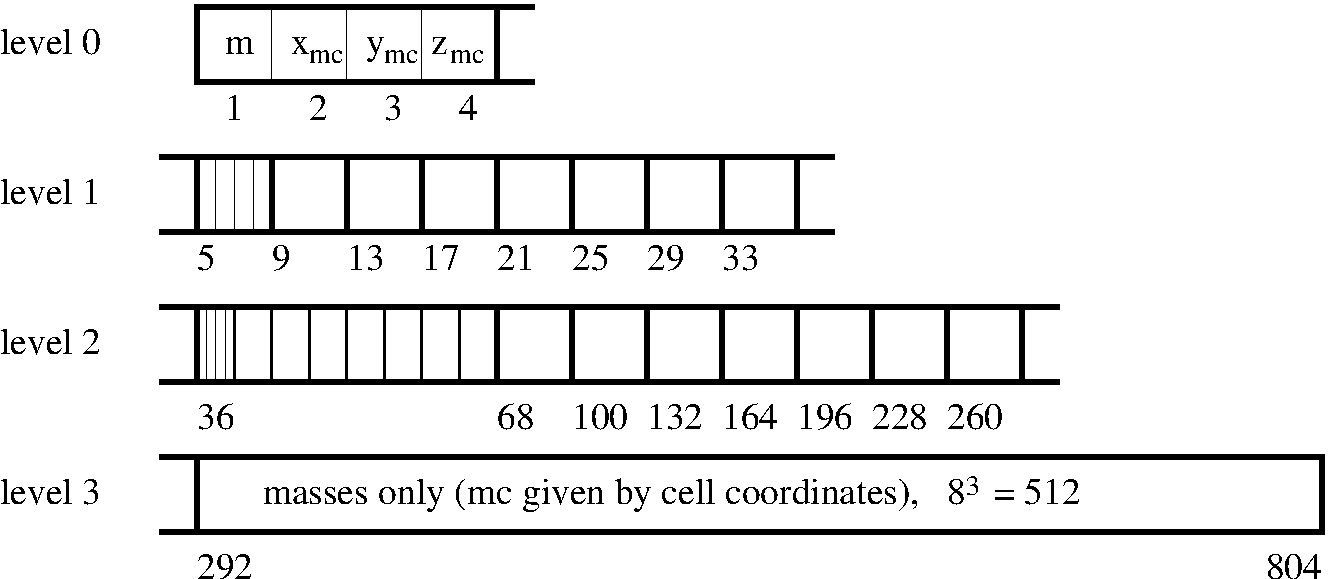
\includegraphics[width=15cm]{tree-in-ram}
\caption{Example of a {block-tree} in case of
\texttt{nxb}=\texttt{nyb}=\texttt{nzb}=8 and in case physical units do not
store any further information to tree nodes (masses and mass centre positions
are included by the tree solver itself).}
\label{fig:btree}
\end{figure}

\textit{Communication of the tree.} Most of the tree data is contained on the
bottom levels in individual {\em block-trees}. In order to save memory and
communication time, only parts of {\em block-trees} that are needed on a given
processor are sent to it. The procedure consists of three steps. In the first
one, a level down to which each {\em block-tree} has to be sent to each
processor is determined. For a given {\em block-tree}, it is done by evaluating
the criterion for the node acceptance (traditionally called multipole acceptance
criterion, shortly MAC) for all blocks on a remote processor, searching for the
maximum level down to which the evaluated node will be needed on a given remote
processor. In the second step, information about the {\em block-tree}
levels which are going to be communicated is sent to all processors. This
information is needed for allocation of arrays in which {\em block-trees} are
stored on remote processors. In the third step, the {\em block-tree} arrays are
allocated, all {\em block-trees} for a given processor are packed into a single
message and the messages are communicated.

The MAC is implemented in subroutine \code{gr\_bhMAC} which includes only a
simple geometrical MAC used also by Barnes \& Hut. The node is accepted for
calculation if
\begin{equation}
\label{eq:stl}
\frac{S_\mathrm{node}}{D} < \mathtt{gr\_bhTreeLimAngle} \ ,
\end{equation}
where $S_\mathrm{node}$ is the node size (defined as the largest edge of the
corresponding cuboid) and $D$ is the distance between the node and the {\em
point-of-calculation}. Additionally, \code{gr\_bhMAC} checks that the {\em
point-of-calculation} is not located within the node itself enlarged by factor
\rpi{Grid/gr\_bhTreeSafeBox}. On the top of that, \code{gr\_bhMAC} calls MACs of 
physical units and the node is accepted only if all criteria are fulfilled.

\textit{Tree walk.} The tree is traversed from the top to the bottom, evaluating
MAC of each node and in case it is not fulfilled, continuing the tree walk with
its children. If the node's MAC is fulfilled, the node is accepted for the
calculation and subroutine \code{gr\_bhBotNodeContrib} or
\code{gr\_bhNodeContrib} is called, depending on whether it is a bottom-most
node (i.e. a single grid cell) or higher node, respectively. These subroutines
only call the corresponding subroutines of physical units (\eg,
\texttt{Gravity\_bhNodeContrib}). This is the most CPU-intensive part of
the tree solver, it usually takes more than $90\%$ of the total tree solver
time. It is completely parallel and it does not include any communication (apart
from sending some statistics to the main processor at the end).

The tree solver includes several implementations of the tree walk. The default
algorithm is the Barnes-Hut like tree walk in which the whole tree is traversed
from the top down to nodes fulfilling MAC for each cell separately. This
algorithm is used in case the runtime parameter \rpi{Grid/gr\_bhUnifiedTreeWalk} is
true (default). If it this parameter is set to false, another algorithm is used
in which instead of walking the whole tree for each cell individually, MAC is at
first evaluated for whole mesh block (interacting with some node). If the node
is accepted and if the node is a parent node (i.e. corresponding to whole mesh
block), the node is accepted for all cells of the block and the contribution of
the node is added to them. However, the node contribution is calculated
separately for each cell, because the distance between the node and individual
cells differs. The third tree walk algorithm is an implementation of the so
called \texttt{SumSquare} MAC described by Salmon \& Warren (1994). The tree is
traversed using the priority queue, taking contribution of the most important
nodes first. This algorithm provides much better error control, however, the
implementation in this code version is highly experimental.

The tree solver supports isolated and periodic boundary conditions that can be
set independently in each direction. In the latter case, when a node is
considered for MAC evaluation and eventually calculation by calling
\api{physics/Gravity/Gravity\_bhNodeContrib}, periodic copies of the
node are checked, and the minimum distance among the node periodic copies is
taken in account. This allows for instance to calculate gravitational potential
with periodic boundary conditions using the Ewald method (see description of the
Gravity unit).


\subsubsection{Tree Poisson solver unit test}

The unit test for the tree gravity solver calculates the gravitational potential
of the Bonnor-Ebert sphere (Bonnor, W. B., 1956, MNRAS, 116, 351) and compares
it to the analytical potential. The density distribution and the analytical
potential are calculated by the python script \texttt{bes-generator.py}. The
simulation setup only reads the file with radial profiles of these quantities
and sets it on the grid. It also normalizes the analytical potential (adds a
constant to it) so that the minimum values of the analytical and numerical
potential are the same. The error of the gravitational potential calculated by
the tree code is stored in the field array PERR (written into the PlotFile). The
maximum absolute and relative errors are written into the log file.


%-------------------------------------------------------------------------------
%\input{GridSolversTreeWunsch.tex}  (old version)
%-------------------------------------------------------------------------------


\subsubsection{Multigrid Poisson solver}
\label{Sec:GridSolversMultigrid}

This section of the  User's Guide is taken from a paper by
Paul Ricker,
``A Direct Multigrid Poisson Solver for Oct-Tree Adaptive Meshes''
 (2008).  Dr. Ricker wrote an original version of this 
multigrid algorithm for \flashx.  The Flash Center adapted it to
\flashx.

Structured adaptive mesh refinement provides some challenges for the
implementation of effective, parallel multigrid methods.  In the case of
patch-based meshes, Huang \& Greengard (2000) presents an algorithm which works by
using the coarse-grid solution to impose boundary values on the fine grid.
Discontinuities in the solution caused by jumps in refinement are resolved
through iterative calculation of the residual and subsequent correction.  While
this is not a multigrid method in the standard sense, it still provides
significant convergence acceleration.

The adaptation of this method to the Flash-X grid structure (Ricker, 2008) requires a few
modifications.  The original formulation required that there be shared points
between the coarse and fine patches.  Contrast this with finite-volume,
nested-cell, cell-averaged grids as used in Flash-X(\figref{Fig:GridSolvers_hgMultigrid_f1}).  This is overcome by the
exchange of guardcells from coarse to fine using monotonic interpolation
(\secref{Sec:gridinterp}) and external boundary extrapolation for the calculation of
the residual.

\begin{figure}[!ht]
\begin{center}
{\leavevmode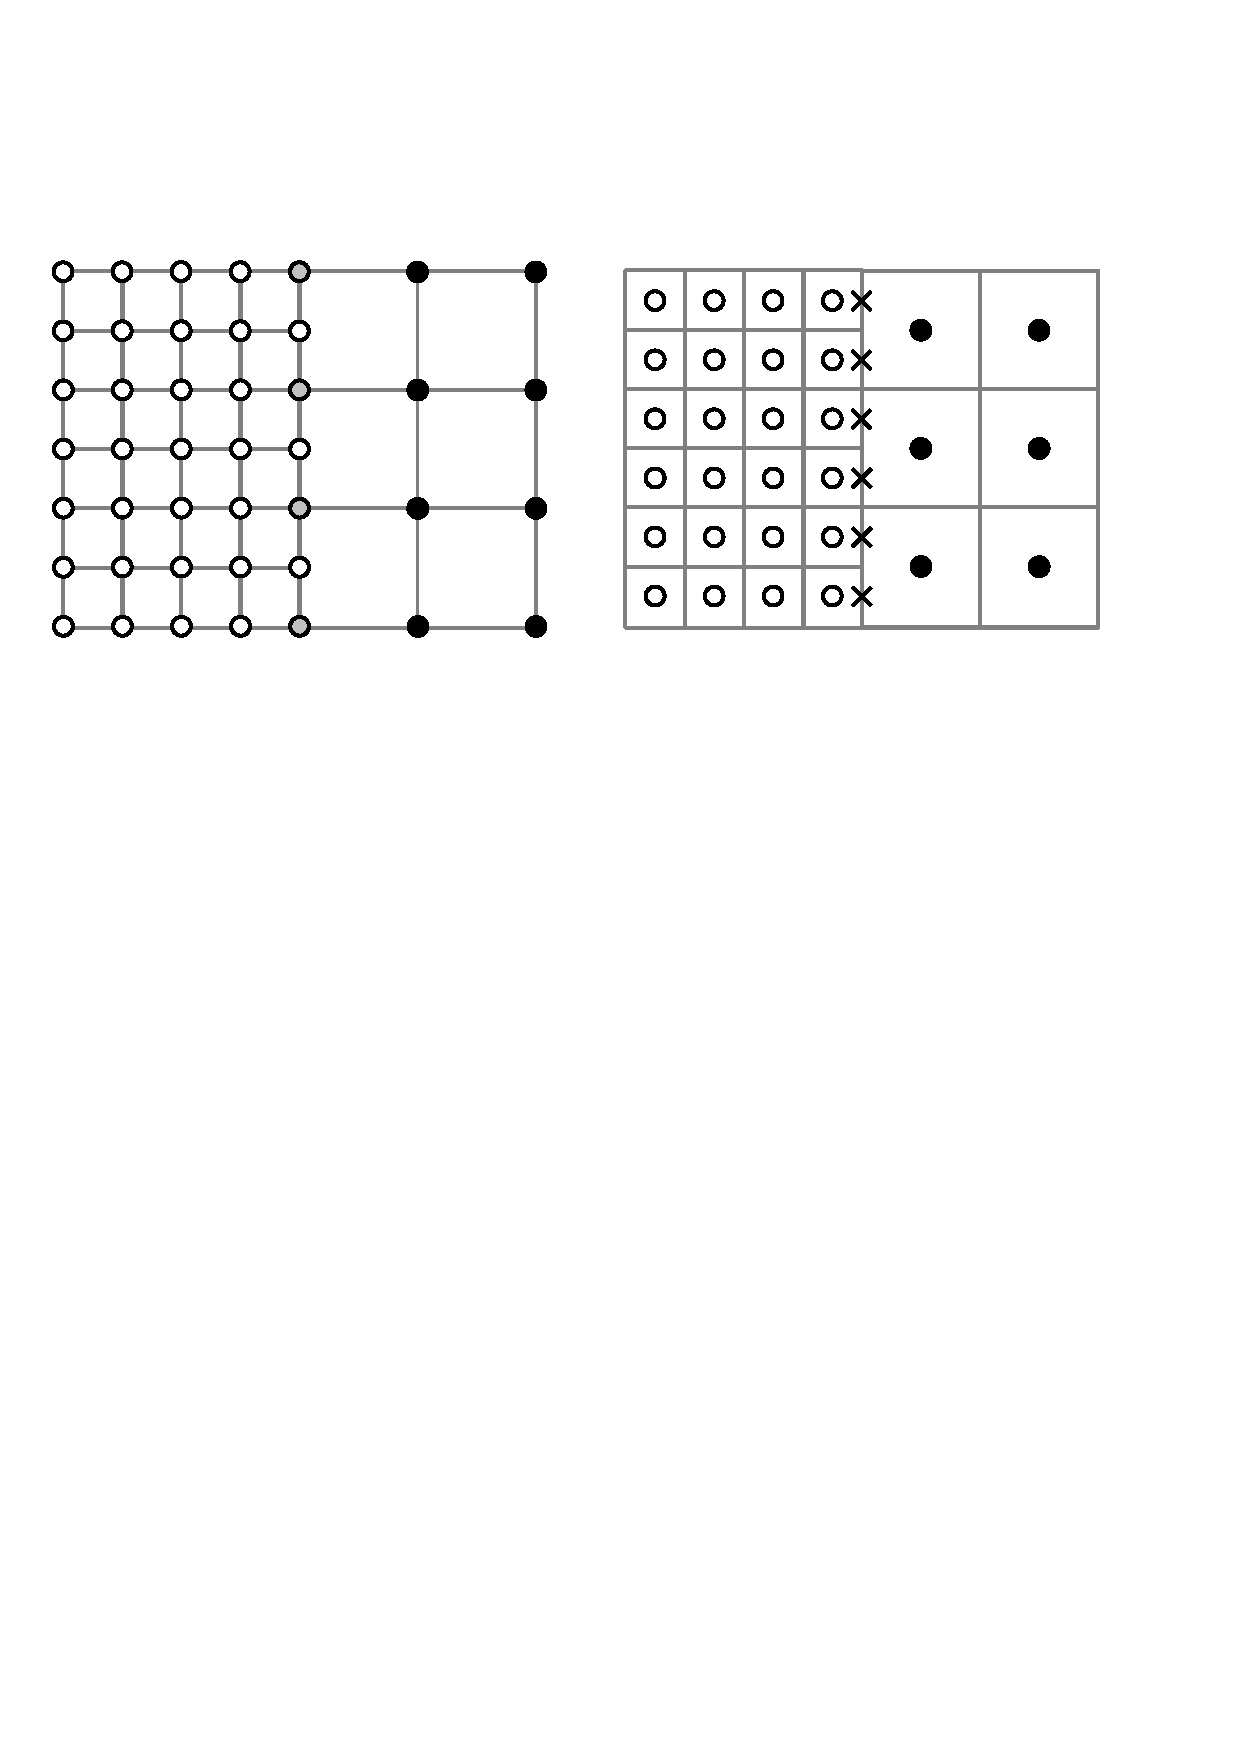
\includegraphics[width=100mm]{GridSolvers_hgMultigrid_f1}}
\end{center}
\caption{\label{Fig:GridSolvers_hgMultigrid_f1} Contrast between jumps of refinement in meshes used in the original paper
(left) and the oct-tree adapted method (right).}
\end{figure}

Another difference between the method of (Ricker 2008) and Huang \& Greengard is
that an oct-tree undoubtedly has neighboring blocks of the same
refinement, while a patch-based mesh would not. This problem is solved through
uniform prolongation of boundaries from coarse-to-fine, with simple relaxation
done to eliminate the slight error introduced between adjacent cells.

One final change between the two methods is that the original computes new
sources at the boundary between corrections, while the propagation here is done
through nested solves on various levels. 

The entire algorithm requires that the PARAMESH grid be reset such that all
blocks at refinement above some level $\ell$ are set as temporarily nonexistent.
This is required so that guardcell filling can occur at only that level,
neglecting blocks at a higher level of refinement.  This requires some global
communication by PARAMESH.

The method requires three basic operators over the solution $\phi$ on the grid:
taking the residual, restricting a fine-level function to coarser-level blocks,
and prolonging values from the coarse level to the faces of fine level blocks in
order to impose boundary values for the fine mesh problems.

The residual is calculated such that: 

\begin{equation}
\label{Eqn:residual}
R({\bf x}) \equiv  4\pi G \rho({\bf x}) - \nabla^2 \tilde\phi({\bf x})\ .
\end{equation}

This is accomplished through the application of the finite difference laplacian,
defined on level $\ell$ with length-scales $\Delta x_\ell$, $\Delta y_\ell$ and
$\Delta z_\ell$.

\begin{eqnarray}  % multiple lines needed in equation
{\cal D}_\ell\tilde\phi^{b\ell}_{ijk} & \equiv &
 {1\over\Delta x_\ell^2}\left(\tilde\phi^{b\ell}_{i+1,jk} -
                              2\tilde\phi^{b\ell}_{ijk} +
                              \tilde\phi^{b\ell}_{i-1,jk}\right)+ 
 {1\over\Delta y_\ell^2}\left(\tilde\phi^{b\ell}_{i,j+1,k} -
                              2\tilde\phi^{b\ell}_{ijk} +
                              \tilde\phi^{b\ell}_{i,j-1,k}\right)  \\
 & & + {1\over\Delta z_\ell^2}\left(\tilde\phi^{b\ell}_{ij,k+1} -
                              2\tilde\phi^{b\ell}_{ijk} +
                              \tilde\phi^{b\ell}_{ij,k-1}\right)\ .
\end{eqnarray}

The restriction operator ${\cal R}_\ell$ for block interior zones $(i,j,k)$ is:
\begin{equation}
({\cal R}_\ell\tilde\phi)^{{\cal P}(c),\ell}_{ijk} \equiv {1 \over {2^d}}
  \sum_{i'j'k'}
  \tilde\phi^{c,\ell+1}_{i'j'k'}\ ,
\end{equation}
where the indices $(i',j',k')$ refer to the zones in block $c$ that lie within
zone $(i,j,k)$ of block ${\cal P}(c)$.  We apply the restriction operator
throughout the interiors of blocks, but its opposite, the prolongation operator
${\cal I}_\ell$, need only be defined on the edges of blocks, because it is only
used to set boundary values for the direct single-block Poisson solver:
\begin{equation}
({\cal I}_\ell\tilde\phi)^{c,\ell+1}_{i'j'k'} \equiv \sum_{p,q,r = -2}^2
                 \alpha_{i'j'k'pqr}\tilde\phi^{{\cal P}(c),\ell}_{i+p,j+q,k+r}
\end{equation}
When needed, boundary zone values are set as for the difference operator.  We
use conservative quartic interpolation to set edge values, then solve with
homogeneous Dirichlet boundary conditions after using second-order
boundary-value elimination.  The coefficients $\alpha$ determine the
interpolation scheme. For the $-x$ face in 3D,
\begin{eqnarray}
\alpha_{1/2,j'k'pqr} &=& \beta_p \gamma_{j'q} \gamma_{k'r} \\
\nonumber
(\beta_p) &=& \left( -{1\over{12}}, {7\over{12}}, {7\over{12}},
                    -{1\over{12}}, 0 \right) \\
\nonumber
(\gamma_{j'q}) &=& \left\{\begin{array}{ll}\displaystyle
                   \left( -{3\over{128}}, {{11}\over{64}},
                                    1, -{{11}\over{64}}, {3\over{128}}\right)
                              & \ \ \ j' {\rm\ odd} \\
                   \displaystyle
                   \left( {3\over{128}}, -{{11}\over{64}},
                                    1, {{11}\over{64}}, -{3\over{128}}\right)
                              & \ \ \ j' {\rm\ even} 
                  \end{array} \right.
\end{eqnarray}
Interpolation coefficients are defined analogously for the other faces.
Note that we use half-integer zone indices to refer to averages over the
faces of a zone; integer zone indices refer to zone averages.

\subsubsection{The direct solver}
\label{Sec:direct solver}

In the case of problems with Dirichlet boundary conditions, a $d$-dimensional
fast sine transform is used.  The transform-space Green's Function for this is:

\begin{equation}
G^\ell_{ijk} = -16\pi G\left[ {1\over{\Delta x_\ell^2}}\sin^2\left({i\pi\over
2n_x}\right) + {1\over{\Delta y_\ell^2}}\sin^2\left({j\pi\over 2n_y}\right) +
{1\over{\Delta z_\ell^2}}\sin^2\left({k\pi\over 2n_z}\right)\right]^{-1}\ .
\end{equation} 

However, to be able to use the block solver in a general fashion, we must be
able to impose arbitrary boundary conditions per-block. In the case of
nonhomogenous Dirichlet boundary values, boundary value elimination may be used
to generalize the solver.  For instance, at the $-x$ boundary:

\begin{equation}
\label{Eqn:bvelim}
\rho_{1jk} \rightarrow \rho_{1jk} - {2\over\Delta x_\ell^2}\phi(x_{1/2},y_j,z_k)\ .
\end{equation}

For periodic problems only the coarsest block must be handled differently; block
adjacency for finer levels is handled naturally.  The periodic solver uses a
real-to-complex FFT with the Green's function:

\begin{equation}
G^\ell_{ijk} = \left\{\begin{array}{ll}\displaystyle {-16\pi G\left[
{1\over{\Delta x_\ell^2}}\sin^2\left({(i-1)\pi\over n_x}\right) + {1\over{\Delta
y_\ell^2}}\sin^2\left({(j-1)\pi\over n_y}\right) + {1\over{\Delta
z_\ell^2}}\sin^2\left({(k-1)\pi\over n_z}\right)\right]^{-1}}\\
\\
                               \hfill i, j, {\rm\ or\ } k \ne 1 \\
\\
\displaystyle
                   0\hfill i = j = k = 1 
                  \end{array} \right.
\end{equation}

This solve requires that the source be zero-averaged; otherwise the solution is
non-unique.  Therefore the source average is subtracted from all blocks.  In
order to decimate error across same-refinement-level boundaries, Gauss-Seidel
relaxations to the outer two layers of zones in each block are done after
applying the direct solver to all blocks on a level.  With all these components
outlined, the overall solve may be described by the following algorithm:

\begin{enumerate}
\item Restrict the source function $4\pi G\rho$ to all levels.  Subtract the
global average for the \code{periodic} case.
\item {\it Interpolation step:} For $\ell$ from 1 to $\ell_{\rm max}$,
      \begin{enumerate}
	\item Reset the grid so that $\ell$ is the maximum refinement level	
 	\item Solve ${\cal D}_\ell \tilde\phi^{b\ell}_{ijk} =
            4\pi G\rho^{b\ell}_{ijk}$ for all blocks $b$ on level $\ell$.
    	\item Compute the residual $R^{b\ell}_{ijk} = 4\pi G\rho^{b\ell}_{ijk} -
            {\cal D}_\ell \tilde\phi^{b\ell}_{ijk}$
    	\item For each block $b$ on level $\ell$ that has children, prolong
            face values for $\tilde\phi^{b\ell}_{ijk}$ onto each child block.
      \end{enumerate}
\item {\it Residual propagation step:} 
      Restrict the residual $R^{b\ell}_{ijk}$ to all levels.
\item {\it Correction step:} Compute the discrete $L_2$ norm of the residual over
      all leaf-node blocks and divide it by the discrete $L_2$ norm of the source
      over the same blocks. If the result is greater than a preset threshold
      value, proceed with a correction step: for each level $\ell$ from 1 to
      $\ell_{\rm max}$,
      \begin{enumerate}
	\item Reset the grid so that $\ell$ is the maximum refinement level
      	\item Solve ${\cal D}_\ell C^{b\ell}_{ijk} =
            R^{b\ell}_{ijk}$ for all blocks $b$ on level $\ell$.
      	\item Overwrite $R^{b\ell}_{ijk}$ with the new residual
            $R^{b\ell}_{ijk} - {\cal D}_\ell C^{b\ell}_{ijk}$ for all blocks
            $b$ on level $\ell$.
      \item Correct the solution on all leaf-node blocks $b$ on level $\ell$:
            $\tilde\phi^{b\ell}_{ijk} \rightarrow \tilde\phi^{b\ell}_{ijk} +
            C^{b\ell}_{ijk}$.
      \item For each block $b$ on level $\ell$ that has children, interpolate
            face boundary values of $C^{b\ell}_{ijk}$ for each child.
      \end{enumerate}
\item If a correction step was performed, return to the residual propagation
      step.
\end{enumerate}

The above procedure requires storage for $\tilde\phi$, $C$, $R$, and $\rho$ on
each block, for a total storage requirement of $4 n_x n_y n_z$ values per
block. Global communication is required in computing the tolerance-based
stopping criterion.


\subsubsection{A Hybrid Poisson Solver: Interfacing PFFT with Multigrid}
\label{PFFTMultigrid}
We can improve the performance of the Multigrid solver in Section
\ref{Sec:GridSolversMultigrid} by replacing single block FFTs with a
parallel FFT at a specified coarse level, where, the coarse level is
any level which is fully refined, i.e. containing blocks that
completely cover the computational domain.  Currently, we
automatically select the maximum refinement level that is fully
refined.

There is load imbalance in the Multigrid solver because each processor
performs single block FFTs on the blocks it owns.  At the coarse
levels there are relatively few blocks compared to available
processors which means many processors are effectively idle during the
coarse level solves.  The introduction of PFFT, and creation of a
hybrid solver, eliminates some of the coarse level solves.


The performance characteristics of the hybrid solver are described in
``Optimization of multigrid based elliptic solver for large scale
simulations in the Flash-X code'' (2012) which is available online at
\url{http://onlinelibrary.wiley.com/doi/10.1002/cpe.2821/pdf}.
Performance results are obtained using the PFFT\_PoissonFD unit test.



\subsection{Using the Poisson solvers}

The \code{GridSolvers} subunit solves the Poisson equation
(\eqref{Eqn:general Poisson}).
Two different elliptic solvers are supplied with Flash-X: a multipole
solver, suitable for approximately spherical source distributions,
and a multigrid solver, which can be used with general source distributions.
The multipole solver accepts only isolated boundary conditions, whereas
the multigrid solver supports Dirichlet, given-value, Neumann,
periodic, and isolated boundary conditions. Boundary conditions for the
Poisson solver are specified using an argument to the 
\api{Grid/Grid_solvePoisson}
routine which can be set from different runtime parameters depending on
the physical context in which the Poisson equation is being solved.
The \code{Grid_solvePoisson} routine is the primary entry point to the Poisson
solver module and has the following interface
\begin{quote}
\code{call Grid_solvePoisson (}{\it iSoln}\code{, }{\it iSrc}\code{, }
{\it bcTypes(6)}\code{, }{\it bcValues(2,6)}\code{, }{\it poisfact}\code{)}~,
\end{quote}
where {\it iSoln} and {\it iSrc} are the integer-valued
indices of the solution and source (density) variables,
respectively. {\it bcTypes(6)} is an integer array specifying the
type of boundary conditions to employ on each of the (up to) 6 sides
of the domain.  Index 1 corresponds to the -x side of the domain, 2 to
+x, 3 to -y, 4 to +y, 5 to -z, and 6 to +z.  The following values are
accepted in the array
\begin{center}
\begin{tabular}{cl}
{\it bcTypes} & Type of boundary condition\\
\hline
0 & Isolated boundaries\\
1 & Periodic boundaries\\
2 & Dirichlet boundaries\\
3 & Neumann boundaries\\
4 & Given-value boundaries\\
\hline
\end{tabular}
\end{center}
Not all boundary types are supported by all solvers.  In this release, {\it
bcValues(2,6)} is not used and can be filled arbitrarily.  Given-value
boundaries are treated as Dirichlet boundaries with the boundary values
subtracted from the outermost interior cells of the source; for this case the
solution variable should contain the boundary values in its first layer of
boundary cells on input to \code{Grid_solvePoisson}.  It should be noted that if
 \Paramesh is used, the values must be set for all levels.  Finally,
{\it poisfact} is real-valued and indicates the value of $\alpha$ multiplying the
source function in  (\eqref{Eqn:general Poisson}).


When solutions found using the Poisson solvers are to be differenced
(\eg, in computing the gravitational acceleration),
it is strongly recommended
that 
%% you use the \code{quadratic\_cartesian/cylindrical/spherical}
%% (quadratic) interpolants supplied  
%% by Flash-X. 
for AMR meshes, quadratic (or better) spatial
interpolation%\index{grid!interpolation}
at fine-coarse boundaries is chosen.  (For PARAMESH,
   this is automatically the case by default, and is handled correctly
   for Cartesian as well as the supported curvilinear geometries.
   But note that the default interpolation implementation may be changed 
   at configuration time with the 
   '\code{-gridinterpolation=}\ldots'%\index{setup!-gridinterpolation@\code{-gridinterpolation}}
   setup option;
   and with the default implementation, the interpolation order may be
   lowered with the \rpi{Grid/interpol_order} runtime parameter.)
If the order of the gridinterpolation of the mesh
is not of at least the same order as the differencing scheme used
in places like \api{physics/Gravity/Gravity_accelOneRow},
unphysical forces will be produced at refinement boundaries. Also, using
constant or linear grid interpolation may cause the multigrid solver to fail
to converge.


\subsubsection{Multipole (original version)}
\label{Sec:GridSolversMultipoleUsing}

The \code{poisson/multipole} sub-module takes two runtime parameters,
listed in \tblref{Tab:multipole parameters}.
Note that storage and CPU costs scale roughly as the square of
\code{mpole\_lmax}, so it is best to use this module only for nearly
spherical matter distributions.
\begin{table}
\caption{ Runtime parameters used with 
\code{poisson/multipole}.}
\label{Tab:multipole parameters} 
\begin{center}
\begin{tabular}{lllp{3in}}
Variable	& Type		& Default	& Description\\
\hline
\code{mpole\_lmax} & integer     & 10        & Maximum multipole moment\\
\code{quadrant}    & logical     & \code{.false.} & Use symmetry to solve a single
                                                  quadrant in 2D axisymmetric
                                                  cylindrical ($r,z$)
                                                  coordinates, instead of a
                                                  half domain.\\
\hline
\end{tabular}
\end{center}
\end{table}



\subsubsection{Multipole (improved version)}
\label{Sec:GridSolversMultipoleImprovedUsing}

To include the new multipole solver in a simulation, the best option
is to use the shortcut \code{+newMpole} at setup command line,
effectively replacing the following setup options :
\begin{codeseg}
-with-unit=Grid/GridSolvers/Multipole_new
-with-unit=physics/Gravity/GravityMain/Poisson/Multipole
-without-unit=Grid/GridSolvers/Multipole
\end{codeseg}
The improved multipole solver currently accepts only two setup parameters, either
one switching on multithreading:
\begin{itemize}
\item
{\bf threadBlockList}: enables multithreaded compilation and execution.
\item
{\bf threadWithinBlock}: enables multithreaded compilation and execution.
\end{itemize}
The names of these two setup parameters are missleading, since there is only one
universal threading strategy used. The use of these two setup parameters is a
temporary solution and will be replaced in near future by only one setup parameter.
\par
The improved multipole solver takes several runtime parameters,
whose functions are explained in detail below, together with comments about expected
time and memory scaling.

\begin{itemize}
\item
\rpi{Grid/mpole\_Lmax}: The maximum angular moment $L$ to be used for the multipole
Poisson solver. Depending on the domain geometry, the memory and time scaling factors
due to this variable alone are: i) 3D cartesian, 3D cylindrical $\rightarrow (L+1)(L+1)$, ii)
3D cartesian axisymmetric, 2D cylindrical, 2D spherical $\rightarrow (L+1)$,
iii) 1D spherical $\rightarrow 1$. Assuming no memory limitations, the multipole
solver is numerically stable for very large $L$ values. Runs up to $L=100$
for 3D cartesian domains have been performed. For 2D geometries, $L=1000$ was the
maximum tested.
\item
\rpi{Grid/mpole\_2DSymmetryPlane}: In 2D coordinates, this runtime parameter
enables the user to specify a plane of symmetry along the radial part of the
domain coordinates. In effect, this allows a reduction of the computational
domain size by one half. The code internally computes the multipole moments as if the
other symmetric part is present, i.e. no memory or execution time savings
can be achieved by this runtime parameter.
\item
\rpi{Grid/mpole\_3DAxisymmetry}: Forces rotational invariance around the main ($z$)
axis in 3D cartesian domains. The assumed rotational invariance in the $(x,y)$
plane effectively cancels all $m\neq 0$ multipole moments and one can restrict
the calculation to the $m=0$ multipole moments only. The time and memory
savings compared to a asymmetric 3D cartesian run is thus about a factor
of $(L+1)$. For 3D cylindrical domains, rotational invariance in the $(x,y)$
plane is equivalent of setting up the corresponding 2D cylindrical domain,
hence this runtime parameter is not honored for 3D cylindrical domains, and
the user is informed about the 3D to 2D cylindrical domain reduction possibility.
\item
\rpi{Grid/mpole\_DumpMoments}: This parameter is meant mainly for debugging purposes.
It prints the entire moment array for each radial bin for each time step.
This option should be used with care and for small problems only. The output
is printed to a text file named '$<$basenm$>$\_dumpMoments.txt', where $<basenm>$
is the base name given for the output files.
\item
\rpi{Grid/mpole\_PrintRadialInfo}: This parameter enables showing all detailed radial
bin information at each time step. This option is especially useful for optimizing
the radial bin sizes. The output is written to the text file '$<$basenm$>$\_printRadialInfo.txt'.
\item
\rpi{Grid/mpole\_IgnoreInnerZone}: Controls switching on/off the radial inner zone.
If it is set .true., the inner zone will not be recognized and all inner zone
radii will be treated statistically. This parameter is meant only for performing
some error analysis. For production runs it should always be at its default value
of false. Otherwise errors will be introduced in calculating the moments near
the expansion center.
\item
\rpi{Grid/mpole\_InnerZoneSize}: The size defining the discrete inner zone. The size
is given in terms of the inner zone smallest (atomic) radius, which is determined
at each time step by analyzing the domain grid structure around the multipolar origin
(expansion center). Only very rarely will this value ever have to be changed. The
default setting is very conservative and only under unusual circumstances
(ex: highly nonuniform grid around the expansion center) this might be necessary.
This value needs to be an integer, as it is used by the code to define dimensions
of certain arrays. Note, that by giving this runtime parameter a large integer
value (> 1000 for domain refinement levels up to 5) one can enforce the code to use
only non-statistical radial bins.
\item
\rpi{Grid/mpole\_InnerZoneResolution}: Defines the inner zone radial bin size for the
inner zone in terms of the inner zone smallest (atomic) radius.
Two inner zone radii will be considered different, if they are more than this
resolution value apart. A very tiny number (for example $10^{-8}$) will result in a complete
separation of all inner zone radii into separate radial bins. The default
value of $0.1$ should never be surpassed, and any attempt to do so will stop the
program with the appropriate information to the user. Likewise with a meaningless
resolution value of 0.
\item
\rpi{Grid/mpole\_MaxRadialZones}: The maximum number of outer radial zones to be used.
In contrast to the inner radial zone, the outer radial zones are much more important
for the user. Their layout defines the performance of the multipole solver both
in cpu time spent and accuracy of the potential obtained at each cell. The
default value of 1 outer radial zone at maximum refinement level leads to high
accuracy, but at the same time can consume quite a bit of memory, especially for full
3D runs. In these cases the user can specify several outer radial zones
each having their own radial bin size determination rule.
\item
\rpi{Grid/mpole\_ZoneRadiusFraction\_n}: The fraction of the maximum domain radius
defining the n-th outer zone maximum radial value. The total number of fractions given
must match the maximum number of outer radial zones specified and the fractions
must be in increasing order and less than unity as we move from the 1st outer zone
upwards. The last outer zone must always have a fraction of exactly 1. If not, the
code will enforce it.
\item
\rpi{Grid/mpole\_ZoneType\_n}: String value containing the outer radial zone type for
the n-th outer zone. If set to 'exponential', the radial equation $r(Q) = s \cdot \Delta r \cdot Q^t$,
defining the upper bound radius of the Q-th radial bin in the n-th outer zone,
is used. If set to 'logarithmic', the radial equation $r(Q) = s \cdot \Delta r \cdot (e^{Qt}-1)/(e^t-1)$ 
is used. In these equations $Q$ is a local radial bin counting index for each outer zone
and $s,t$ are parameters defining size and growth of the outer zone radial bins
(see below).
\item
\rpi{Grid/mpole\_ZoneScalar\_n}: The scalar value $s$ in the n-th outer radial zone equation
$r(Q) = s \cdot \Delta r \cdot Q^t$ or $r(Q) = s \cdot \Delta r \cdot (e^{Qt}-1)/(e^t-1)$. The
scalar is needed to be able to increase (or decrease) the size of the first radial
bin with respect to the default smallest outer zone radius $\Delta r$.
\item
\rpi{Grid/mpole\_ZoneExponent\_n}: The exponent value $t$ in the n-th outer radial zone
equations $r(Q) = s \cdot \Delta r \cdot Q^t$ or $r(Q) = s \cdot \Delta r \cdot (e^{Qt}-1)/(e^t-1)$.
The exponent controls the growth (shrinkage) in size of each radial bin with increasing bin index.
For the first equation, growing will occur for $t>1$, shrinking for $t<1$ and same size
for $t=1$. For the logarithmic equation, growing will occur for $t>0$, shrinking for
$t<0$, but the same size option $t=0$ will not work because the denominator becomes
undefined. The same size option must hence be treated using the exponential outer zone
type choice.
\item
{\bf Runtime parameter types, defaults and options}: 
\begin{center}
\begin{tabular}{llll}
Parameter & Type & Default & Options \\
\hline
\rpi{Grid/mpole\_Lmax}                      & integer & 0     & $>0$    \\
\rpi{Grid/mpole\_2DSymmetryPlane}           & logical & false & true    \\
\rpi{Grid/mpole\_3DAxisymmetry}             & logical & false & true    \\
\rpi{Grid/mpole\_DumpMoments}               & logical & false & true    \\
\rpi{Grid/mpole\_PrintRadialInfo}           & logical & false & true    \\
\rpi{Grid/mpole\_IgnoreInnerZone}           & logical & false & true    \\
\rpi{Grid/mpole\_InnerZoneSize}             & integer & 16    & $>0$    \\
\rpi{Grid/mpole\_InnerZoneResolution}       & real    & 0.1   & less than $0.1$ and $>0.0$ \\
\rpi{Grid/mpole\_MaxRadialZones}            & integer & 1     & $>1$    \\
\rpi{Grid/mpole\_ZoneRadiusFraction\_n}     & real    & 1.0   & less than $1.0$ and $>0.0$ \\
\rpi{Grid/mpole\_ZoneType\_n}               & string  & ''exponential''   & ''logarithmic'' \\
\rpi{Grid/mpole\_ZoneScalar\_n}             & real    & 1.0   & $>0.0$  \\
\rpi{Grid/mpole\_ZoneExponent\_n}           & real    & 1.0   & $>0.0$ (exponential) \\
                                 & real    &   -   & any $\neq 0$ (logarithmic)
\end{tabular}
\end{center}
\end{itemize}


\subsubsection{Tree Poisson solver}
\label{Sec:GridSolversBHTreeUsing}

The tree gravity solver can be included by \code{setup} or a \code{Config} file by
requesting

\bigskip

\texttt{physics/Gravity/GravityMain/Poisson/BHTree}

\bigskip

The current implementation works only in 3D Cartesian coordinates, and blocks
have to be logically cubic (\ie, \texttt{nxb}=\texttt{nyb}=\texttt{nzb}).
Physical dimensions of blocks can be arbitrary, however, some multipole
acceptance criteria can provide inaccurate error estimates with non-cubic
blocks. The computational domain can have arbitrary dimensions, and there can be
more blocks with \texttt{lrefine}=1 (\ie, \texttt{nblockx}, \texttt{nblocky} and
\texttt{nblockz} can have different values).

Runtime parameters \rpi{Grid/gr\_bhPhysMACTW} and \rpi{Grid/gr\_bhPhysMACComm}
control whether MACs of physical units are used in tree walk and communication,
respectively. If one of them (or both) is set \texttt{.false.}, only purely geometric
MAC is used for a corresponding part of the tree solver. It is not allowed to
set \rpi{Grid/gr\_bhPhysMACTW} = \texttt{.false.} and \rpi{Grid/gr\_bhPhysMACComm} =
\texttt{.true.}.

Runtime parameter \rpi{Grid/gr\_bhTreeLimAngle} allows to set the limit opening
angle for the purely geometrical MAC. Another condition controlling the
acceptance of the node for the calculations is that the {\em point-of-calculation}
must lie out of the box obtained by increasing the considered node by factor
\rpi{Grid/gr\_bhTreeSafeBox}.

Parameter \rpi{Grid/gr\_bhUseUnifiedTW} controls whether the Barnes-Hut like tree
walk algorithm is used (\texttt{.true.}) or whether an alternative algorithm is
used which checks the MAC only once for whole block for interactions with parent
blocks (\texttt{.false.}; see 8.10.2.4 for more details). The latter one is $10
- 20\%$ faster, however, it may lead to higher errors at block boundaries, in
particular if the gravity modules calculates the potential which is
subsequently differentiated to obtain gravitational acceleration. The tree walk
algorithm base on the priority queue is used if \code{grv\_bhMAC} is set to
\texttt{"SumSquare"}.

\bigskip

\begin{tabular}{|l|l|l|l|}
\hline
Variable & Type & Default & Description \\
\hline
\rpi{Grid/gr\_bhPhysMACTW}    & logical & .false. & whether physical MAC should be used in tree walk\\
\hline
\rpi{Grid/gr\_bhPhysMACComm}  &  logical & .false. & whether physical MAC should be used in communication\\
\hline
\rpi{Grid/gr\_bhTreeLimAngle} & real & $0.5$ & limiting opening angle\\
\hline
\rpi{Grid/gr\_bhTreeSafeBox}   & real & $1.2$ & relative size of restricted volume around node where the\\
                               &      &       & point-of-calculation is not allowed to be located\\
\hline
\rpi{Grid/gr\_bhUseUnifiedTW}   & logical  & .true.  & whether Barnes-Hut like tree walk algorithm should be used \\
\hline
\rpi{Grid/gr\_bhTWMaxQueueSize} & integer & .true.  & maximum length of the priority queue\\
\hline
\end{tabular}




\subsubsection{Multigrid}
\label{Sec:GridSolversMultigridUsing}

The \code{Grid/GridSolvers/Multigrid} module is appropriate for general source
distributions.  It solves Poisson's equation for 1, 2, and 3 dimensional
problems with Cartesian geometries.  It only supports the \Paramesh
Grid with one block at the coarsest level. For any other mesh
configuration it is advisable to use the hybrid solver, which switches
to a uniform grid exact solve when the specified level of coarsening
has been achieved. In most use cases for Flash-X, the multigrid solver
will be used to solve for Gravity (see: \secref{chp:Gravity}). It may
be included by \code{setup} or
\code{Config} by including:
\begin{codeseg}
physics/Gravity/GravityMain/Poisson/Multigrid
\end{codeseg}

The multigrid solver may also be included stand-alone using:
\begin{codeseg}
Grid/GridSolvers/Multigrid
\end{codeseg}

In which case the interface is as described above.  The supported boundary
conditions for the module are periodic, Dirichlet, given-value, and isolated.
Due to the nature of the FFT block solver, the same type of boundary condition
must be used in all directions.  Therefore, only the value of {\it bcTypes(1)}
will be considered in the call to \code{Grid_solvePoisson}.

The multigrid solver requires the use of two internally-used grid variables:
\code{isls} and \code{icor}.  These are used to store the calculated residual and solved-for
correction, respectively.  If it is used as a Gravity solver with isolated
boundary conditions, then two additional grid variables, \code{imgm} and
\code{imgp}, are used to store the image mass and image potential.  

\begin{center}
\begin{longtable}{lllp{2.25in}}

\caption{ \label{Tab:multigrid parameters} Runtime parameters used with
\code{Grid/GridSolvers/Multigrid}.} \\

Variable	& Type		& Default	& Description\\
\hline
\rpi{Grid/mg_MaxResidualNorm}
                & real          & $1\times 10^{-6}$  & Maximum ratio of the norm
                 of the residual to that of the right-hand side\\
\rpi{Grid/mg_maxCorrections}
                & integer & 100 & Maximum number of iterations to take\\
\rpi{Grid/mg_printNorm} & real & \code{.true.} & Print the norm ratio per-iteration\\
\rpi{Grid/mpole_lmax} & integer & 4 & The number of multipole moments used in the
isolated case\\
\hline

\end{longtable}
\end{center}

\subsubsection{Hybrid (Multigrid with PFFT)}
\label{Sec:GridSolversHybridUsing}

The hybrid solver can be used in place of the Multigrid solver for
problems with
\begin{itemize}
\item all-periodic
\item 2 periodic and 1 Neumann
\item 1 periodic and 2 Neumann
\end{itemize}
boundary conditions, if the default PFFT solver variant 
(called DirectSolver) is used.  
To use the hybrid solver in this way, add
\code{Grid/\-GridSolvers/\-Multigrid/\-PfftTopLevelSolve} to your
setup line or request the solver in your Simulation Config file (see
e.g. unitTest/PFFT\_PoissonFD).  The following setup lines create a
unit test that uses first the hybrid solver and then the standard
Multigrid solver

\begin{codeseg}
./setup unitTest/PFFT_PoissonFD -auto -3d -parfile=flash_pm_3d.par -maxblocks=800 +noio

./setup unitTest/PFFT_PoissonFD -auto -3d -parfile=flash_pm_3d.par -maxblocks=800 +noio
--without-unit=Grid/GridSolvers/Multigrid/PfftTopLevelSolve
--with-unit=Grid/GridSolvers/Multigrid
\end{codeseg}

It is also possible to select a different PFFT solver variant. In that case,
different combinations of boundary conditions for the Poisson problem may be
supported. 
The \code{HomBcTrigSolver} variant supports the largest set of
combinations of boundary conditions.
Use the \code{PfftSolver} setup variable to choose a variant.
Thus, appending \code{PfftSolver=HomBcTrigSolver} to the \code{setup}
chooses the \code{HomBcTrigSolver} variant.
When using the hybrid solver with the PFFT variants \code{HomBcTrigSolver} or
\code{SimplePeriodicSolver},
the runtime parameter \rpi{Grid/gr_pfftDiffOpDiscretize} should be set to 1.


The \code{Multigrid} runtime parameters given in the previous section also apply.


\subsection {HYPRE}
As a part of implicit time advancement we end up with a system of equations that needs to be solved at every time 
step. In \flashx the HYPRE linear algebra package is used to solve
these systems of equations. Therefore it is necessary to install Hypre
if this capability of Flash-X is to be used.\\

\api{Grid/Grid\_advanceDiffusion} is the API function which solves the system of equations. This API is provided by both
the split and unsplit solvers. The unsplit solver uses HYPRE to solve the system of equations and split solver does
a direct inverse using Thomas algorithm. Note that the split solver relies heavily on PFFT infrastructure
for data exchange and a significant portion of work in split \code{Grid\_advanceDiffusion} involves PFFT routines. In the 
unsplit solver the data exchange is implicitly done within HYPRE and is hidden. \\

The steps in unsplit \code{Grid\_advanceDiffusion} are as follows:
\begin{itemize}
\item {Setup HYPRE grid object}
\item {Exchange Factor B}
\item {Set initial guess}
\item {Compute HYPRE Matrix M such that B = MX}
\item {Compute RHS Vector B}
\item {Compute matrix A}
\item {Solve system AX = B}
\item {Update solution (in \flashx)} \\
\end{itemize} 

Mapping UG grid to HYPRE matrix is trivial, however mapping PARAMESH grid to a HYPRE matrix can be quite complicated. The 
process is simplified using the grid interfaces provided by HYPRE.
\begin{itemize}
\item {Struct Grid interface}
\item {SStruct Grid interface}
\item {IJ System interface}
\end{itemize} 

The choice of an interface is tightly coupled to the underlying grid on which the problem is being solved. We have chosen the SSTRUCT 
interface as it is the most compatible with the block structured AMR mesh in \flashx. Two terms commonly used in HYPRE terminology 
are part and box. We define these terms in equivalent \flashx terminology. A HYPRE box object maps directly to a leaf block in \flashx. 
The block is then defined by it's extents. In \flashx this information can be computed easily using a combination of \code{Grid\_getBlkCornerID} 
and \code{Grid\_getBlkIndexLimits}.All leaf blocks at a given refinement level form a HYPRE part. So number of parts in a typical 
\flashx grid would be give by,  \\

\code{nparts = leaf\_block(lrefine\_max) - leaf\_block(lrefine\_min) + 1} \\

So, if a grid is fully refined or UG, nparts = 1. However, there could still be more then one box object. \\

Setting up the HYPRE grid object is one of the most important step of the solution process. We use the SSTRUCT interface 
provided in HYPRE to setup the grid object. Since the HYPRE Grid object is mapped directly with \flashx grid, whenever the 
\flashx grid changes the HYPRE grid object needs to be updated. Consequentlywith AMR the HYPRE grid setup might happen multiple times. \\

Setting up a HYPRE grid object is a two step process, 
\begin{itemize}
\item Creating stenciled relationships.
\item Creating Graph relationships.
\end{itemize}

Stenciled relationships typically exist between leaf blocks at same refinement level (intra part) and graph relationships exist 
between leaf blocks at different refinement levels (inter part). The
fine-coarse boundary is handled in such a way that fluxes are
conserved at the interface (see \chpref{Chp:diffuse} for details). UG
does not require any graph relationships. \\

Whether a block needs a graph relationship depends on the refinement
level of it's neighbor. While this information is not directly
available in PARAMESH, it is possible to determine whether the block
neighbor is coarser or finer. Combining this information with the
constraint of at best a factor of two jump in refinement at block
boundaries, it is possible to compute the 
part number of a neighbor block, which in turn determines whether we need a graph. Creating a graph involves creating a link between all the cells on
the block boundary. \\

Once the grid object is created, the matrix and vector objects are
built on the grid object. The diffusion solve needs uninterpolated data from 
neighbor blocks even when there is a fine-coarse boundary, therefore
it cannot rely upon the guardcell fill process.
 A two step process is used to handle this situation, \\

\begin{itemize}
\item {Since HYPRE has access to X(at n, \ie, initial guess), the RHS vector B can be computed as MX where M is a modified Matrix.}
\item {Similarly the value of Factor B can be shared across the fine-coarse boundary by using \\
\code{Grid\_conserveFluxes},the fluxes need to be set in a intuitive to way to achieve the desired effect.} \\
\end{itemize}

With the computation of Vector B (RHS), the system can be solved using HYPRE and UNK can be updated. \\

\subsubsection{HYPRE Solvers}
\label{Sec:Hypre Solvers}
In \flashx  we use the HYPRE PARCSR storage format as this exposes the maximum number of iterative solvers. 

\begin{center}
\begin{longtable}{ll}
\caption{ \label{Tab:HYPRE solver types} Solvers, Preconditioners combinations used with \code{Grid/GridSolvers/HYPRE}.} \\
Solver        & Preconditioner  \\
\hline
PCG & AMG, ILU(0) \\
BICGSTAB & AMG, ILU(0) \\
GMRES & AMG, ILU(0) \\
AMG & - \\
SPLIT & - \\
\hline
\end{longtable}
\end{center}

{\bf Parallel runs:} One issue that has been observed is that there is a difference in the results produced by HYPRE using one or 
more processors. This would most likely be due to use of CG (krylov subspace methods), which involves an MPI\_SUM over the 
dot product of the residue. We have found this error to be dependent on the type of problem. One way to get across this problem is to use 
direct solvers in HYPRE like SPLIT. However we have noticed that direct solvers tend to be slow. THe released code has
an option to use the SPLIT solver, but this solver has not been extensively tested and was used only for internal debugging 
purposes and the usage of the HYPRE SPLIT solver in \flashx is purely experimental. \\ 

{\bf Customizing solvers:} HYPRE exposes a lot more parameters to tweak the solvers and preconditioners mentioned above. We have only used those 
which are applicable to general diffusion problems. Although in general these settings might be good enough it is by no means complete and 
might not be applicable to all class of  problems. Use of additional HYPRE parameters might require direct manipulation of \flashx code. \\

{\bf Symmetric Positive Definite (SPD) Matrix:}
PCG has been noticed to have convergence issues which might be related to (not necessarily),
\begin{itemize}
\item {A non-SPD matrix generated due to round of errors (only).} \\
\item {Use of BoomerAMG as PC (refer to HYPRE manual).} \\
\end{itemize}

The default settings use PCG as the solver with AMG as preconditioner. The following parameters 
can be tweaked at run time, \\

\begin{center}
\begin{longtable}{lllp{2.25in}}
\caption{ \label{Tab:HYPRE solver  parameters} Runtime parameters used with \code{Grid/GridSolvers/HYPRE}.} \\
Variable        & Type          & Default       & Description\\
\hline
\code{gr\_hyprePCType}
                & string          & \code{"hypre\_amg"}  & Algebraic Multigrid as Preconditioner \\
\code{gr\_hypreMaxIter}
                & integer & 10000 & Maximum number of iterations\\
\code{gr\_hypreRelTol} & real & $1\times 10^{-8}$ &  Maximum ratio of the norm
                 of the residual to that of the initial residue\\
\code{gr\_hypreSolverType} & string & \code{"hypre\_pcg"} & Type of linear solver, Preconditioned Conjugate gradient \\
\code{gr\_hyprePrintSolveInfo} & boolean & FALSE & enables/disables some basic solver information (for e.g number of iterations) \\
\code{gr\_hypreInfoLevel} & integer & 1 & Verbosity level of solver diagnostics (refer HYPRE manual). \\
\code{gr\_hypreFloor} & real & $1\times 10^{-12}$ & Used to floor the end solution. \\
\code{gr\_hypreUseFloor} & boolean & TRUE & whether to apply {gr\_hypreFloor} to floor results from HYPRE. \\
\hline
\end{longtable}
\end{center}


